\documentclass[11pt]{amsart}
\usepackage{placeins}
\usepackage{graphicx}
\usepackage{hyperref}
\usepackage{longtable}
\title{Optics Simulations for PREX and CREX - G4MC}
\author{Nickie Hirlinger Saylor}%, Seamus Riordan, Robert Michaels, Dustin McNaulty, Kent Pacshe, Guido Urciuoli, Jixie Zhang}

\begin{document}
\maketitle

\begin{center}
\today
\end{center}

\begin{abstract}
We present set of dedicated optics studies for PREX II and CREX using the HRS in Hall A at Jefferson Lab. We discuss the past use of legacy code to study these topics, and the replacement of this code by a modern, unified C++/GEANT4 code, G4MC, a framework originally designed by Jixie Zhang, and expanded by Nickie. We demonstrate that this simulation produces results that are consistant with legacy simulations, and more importantly, reproduces features seen in experimental data in Hall A. We summarize the studies that have been carried out by this tool, and enumerate other studies we wish to carry out in the near future. We will also discuss possible improvements and expansions of G4MC. 
\end{abstract}

\section{Objectives}

A basic simulation of the optical system of Hall A, namely, the septum + HRS (QQDQ) system, is desirable. The ability to predict and study the trajectories of electrons from the target and through the septum + HRS system to our quartz detectors will allow us to answer several essential questions regarding both PREX II and CREX experiments:

\begin{enumerate}
  \item The feasibility of the experiment by determination of the Figure of Merit, and its sensitivity to beam energy
  \item The study of acceptance, especially the effect of replacing the first quadrupole magnet (Q1) with a non-superconducting ``SOS'' magnet
  \item The study of the change in resolution due to the same
  \item The design of collimators for the entrance to Q1, and determination if both experiments may use the same collimator
  \item The engineering ``keep-out'' regions for the experiments
  \item The electron distributions at the focal plane, which determine detector footprints
  \item The optimization of spectrometer tune, for CREX
  \item The effect of poletip scattering
\end{enumerate}

Each of these items will be carefully defined and expanded upon in later sections.

\newpage
\section{Historical Overview}

The original state of simulations was carried out primarily by the use of three separate programs: SNAKE, MUDIFI, and HAMC. SNAKE and MUDIFI are legacy FORTRAN programs. HAMC is a C++/ROOT program.

\subsection{SNAKE}

SNAKE is a raytracing program written by Pascal Vernin in 1986. It is a program written in FORTRAN. In a directive file, one declares a set of overlapping volumes, each with a defined geometry and magnetic property, such as: quad entrance fringe, quad exit fringe, dipole, drift, et c. One may interactively, or by batch, input a series of ingoing particles into the system. SNAKE computes the trajectories of these particles via raytracing, and outputs a the position and angle of particles at various endplanes, which may be defined by the user.

A basic SNAKE plot.

\subsection{MUDIFI}

MUDIFI, or (MU)lti-(DI)mensional-(FI)t-program, is a program written at CERN by Rene Brun et al. in 1977. It is a program written in FORTRAN. The output of the SNAKE program, listed above, it inputed into the fitting program. The bundles of rays output by SNAKE are fit to polynomials which output final positions and angles of trajectories at various endplanes, given initial positions and angles at the target. These output functions are in FORTRAN, and I will refer to them as ``FORTRAN Transport Functions'' in this document.

\subsection{HAMC}

HAMC, or (H)all (A) (M)onte (C)arlo is a program written by Robert Michaels, and is currently maintained. It is a program written in C++. Particles are generated with an appropriate cross section at the target, and inputed into the FORTRAN Transport Functions, output by MUDIFI. In this way, given initial positions and angles at the target, various optics properties of the septum + HRS system can be studied.

\subsection{Outlook on SNAKE-MUDIFI-HAMC System}

While the SNAKE-MUDIFI-HAMC system of studying optics is effective and predictive, there are numerous difficulties which are readily presented. The first is the relative complexity of the system. There are three seperate programs, which are each challenging to run effectively without error. Additionally, two of the programs are written in FORTRAN, which is less portable, and increasingly a language which younger scientists do not read or write. Finally, quick changes in magnetic settings necessitate rerunning the three separate programs from the beginning. This process is lengthly, and historically required multiple experienced users to operate.

A need quickly developed for a program which incorporates the functions of all three programs, SNAKE-MUDIFI-HAMC, without intermediate steps, allowing for quick configuration changes in magnetic field settings, written in a modern language using well-known and -used libraries.

\newpage
\section{G4MC - A Modern Simulation for Optics Studies}

The unification of the function of SNAKE-MUDIFI-HAMC was accomplished via the development of a C++/GEANT4 program called G4MC, or (G)EANT(4) (M)onte (C)arlo. The use of GEANT4 allows for an easy definition of septum + HRS geometry, magnetic fields, and sensitive detectors. The behavior of electrons in magnetic fields is computed via raytracing directly within the program, allowing for quick changes in magnetic field, and bypassing the need for FORTRAN Transport Functions. A generator with rejection sampling was utilized to generate events with either ${}^{48}$Ca and ${}^{208}$Pb cross sections. The particles which cross planes, defined by the user, and recorded along with their positions and angles, and are output to root file which may be analyzed and processed by the user.

The code may be accessed via GitHub:

\url{https://github.com/HirlingerSaylor/G4MC}

\FloatBarrier
\begin{figure}
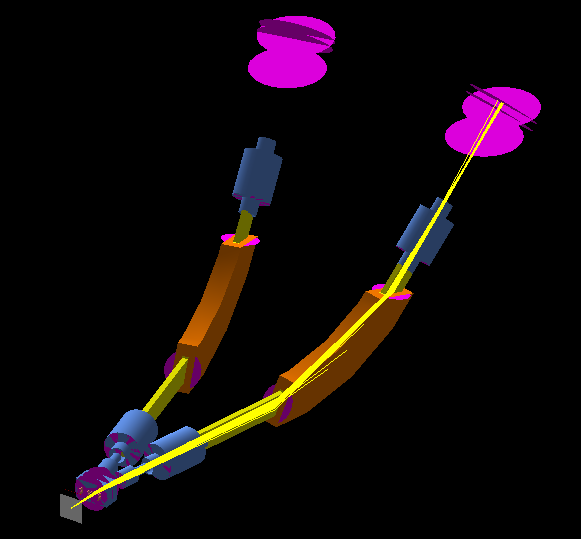
\includegraphics[width=0.75\textwidth]{plots/traj.png}
\caption{A snapshot of G4MC simulations visualization, with 100 electron events travelling through the right HRS. The geometry of the magnetic elements, the target, as well as the sensitive detectors corresponding to the VDCs and quartz detectors may be seen.}
\end{figure}
\FloatBarrier

\newpage
\section{Certification of G4MC}

In order to ``certify'' that our simulation is truly predictive, we have benchmarked it to both the results of the previous simulations suite, SNAKE-MUDIFI-HAMC, and more importantly, to experimental data from Hall A at JLab.

We emphasize that this entire document employs transport coordinate convention, where $x$, is the vertical position, downwards, $\theta$ is the vertical angle, downwards, $y$ is the horizontal position, to the left, and $\phi$ is the horizontal angle to the left, $z$ is in the direction of the central trajectory, and $\delta$ is the fractional momentum difference.

\subsection{Reproduction of SNAKE-MUDIFI-HAMC Results}

Our first step in simulation certification is to compare the results of G4MC with the results of SNAKE. We have done this by sending electrons through the septum + HRS system for both simulations, and comparing the results. Initial conditions may be given at the target for a single track, such as $x=0$, $\theta=0$, $y=0$, $\phi=0$, $\delta=0$, and the resultant variables from each simulation can be compared at various later planes, e.g. the exit of the dipole, or at the focal plane. This was accomplished by imposing various initial conditions by varying each variable independantly, such as $x=2\text{ cm}$, $\theta=0$, $y=0$, $\phi=0$, $\delta=0$. The following plots demonstrate that the optical behavior of the magnetic elements is well reproduced in G4MC.

The complete, interactive study may be found here:

\url{http://hirlinger-saylor.com/research/HallA/optics/matrix/matrix.html}


\FloatBarrier
\begin{figure}
\begin{center}
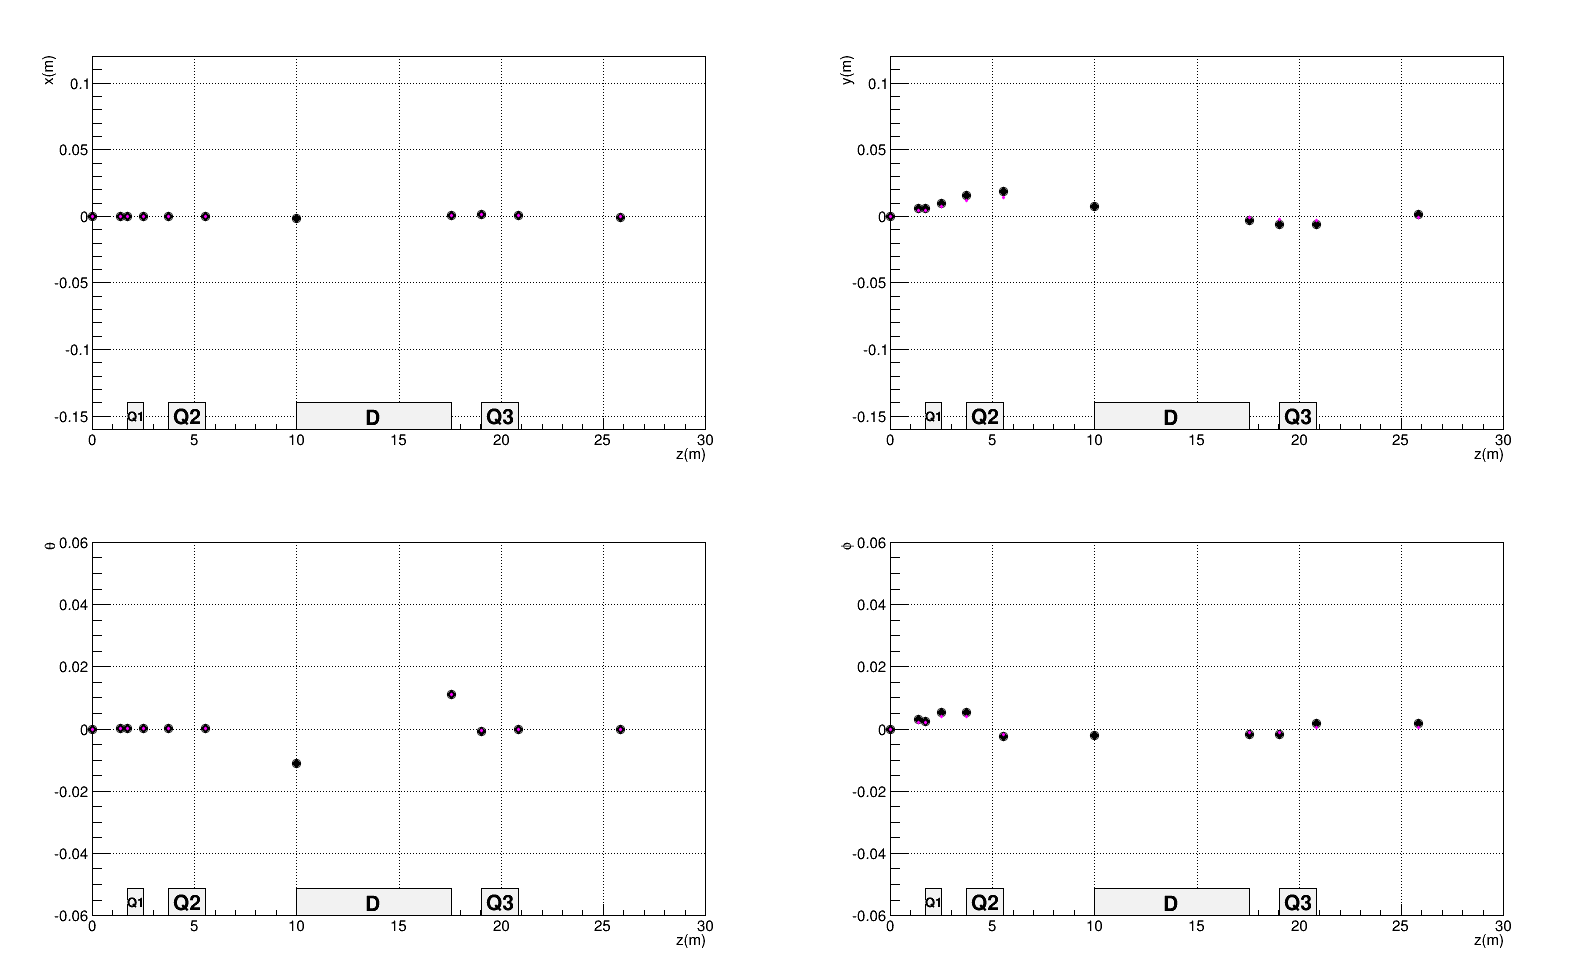
\includegraphics[width=0.95\textwidth]{plots/pres_matrix_x_3.png}
\end{center}
\caption{The central trajectory through the HRS. In the upper left, transport $x$, in the upper right, transport $y$, in the lower left, transport $\theta$, and in the lower right, tranport $\phi$, all as a function of z. The large black points are the results of G4MC. The smaller, superimposed magenta points are the results of SNAKE.}
\end{figure}

\begin{figure}
\begin{center}
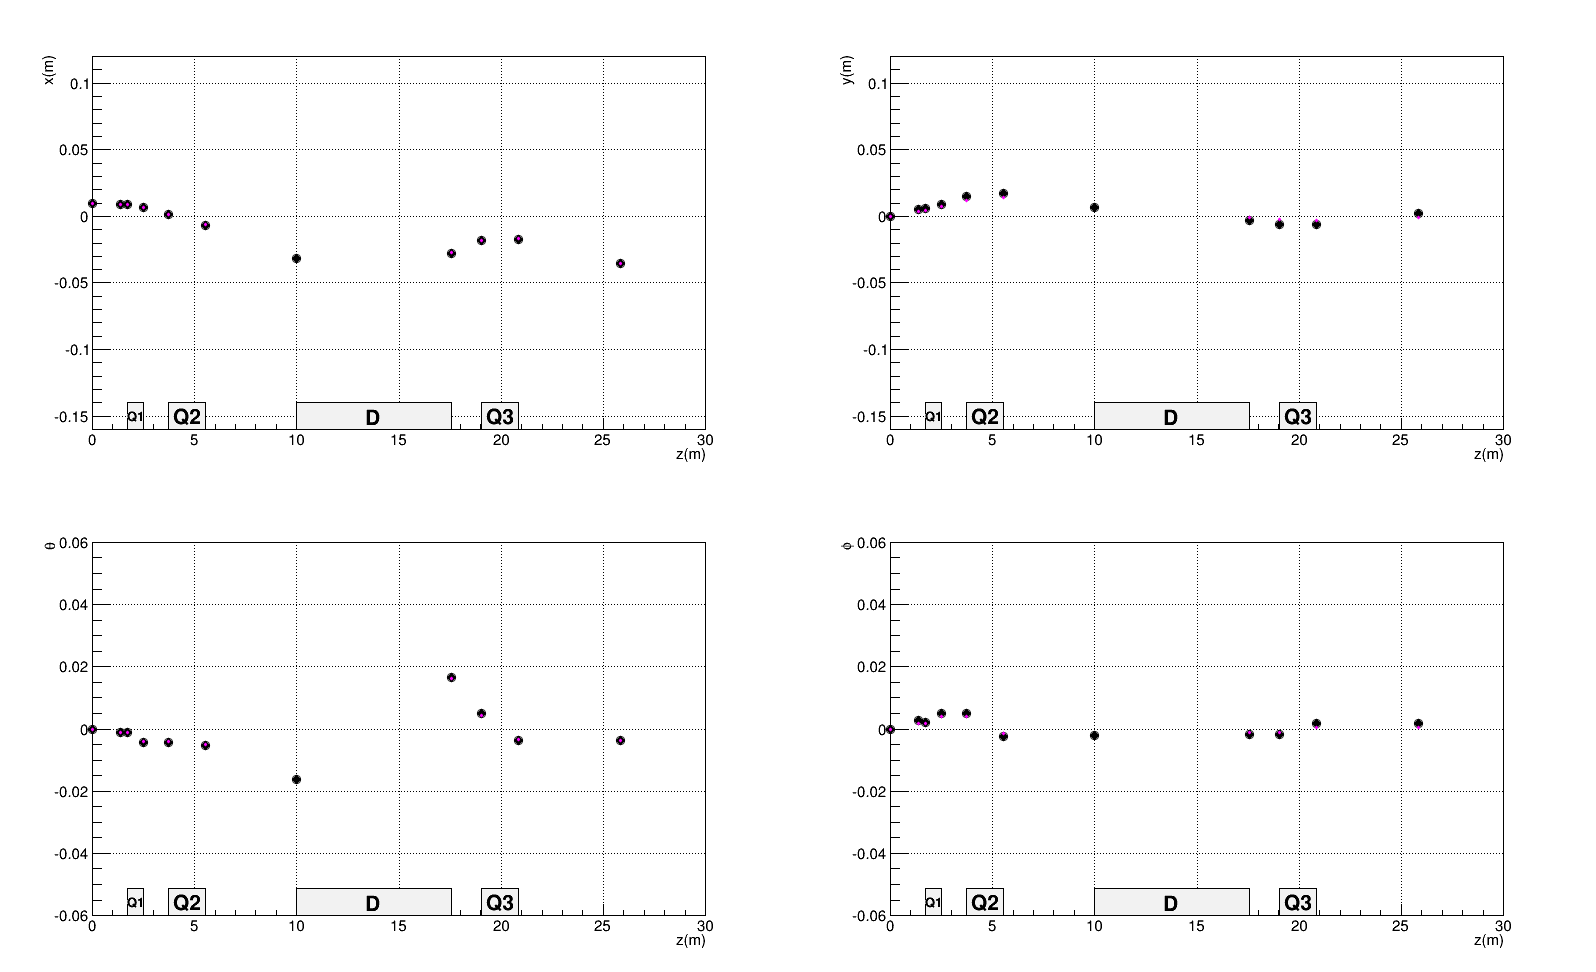
\includegraphics[width=0.95\textwidth]{plots/pres_matrix_x_4.png}
\end{center}
\caption{The results of sending an electron through the HRS with initial target variable $x=1\text{ cm}$, and all other variables 0. In the upper left, transport $x$, in the upper right, transport $y$, in the lower left, transport $\theta$, and in the lower right, tranport $\phi$, all as a function of z. The large black points are the results of G4MC. The smaller, superimposed magenta points are the results of SNAKE.}
\end{figure}

\begin{figure}
\begin{center}
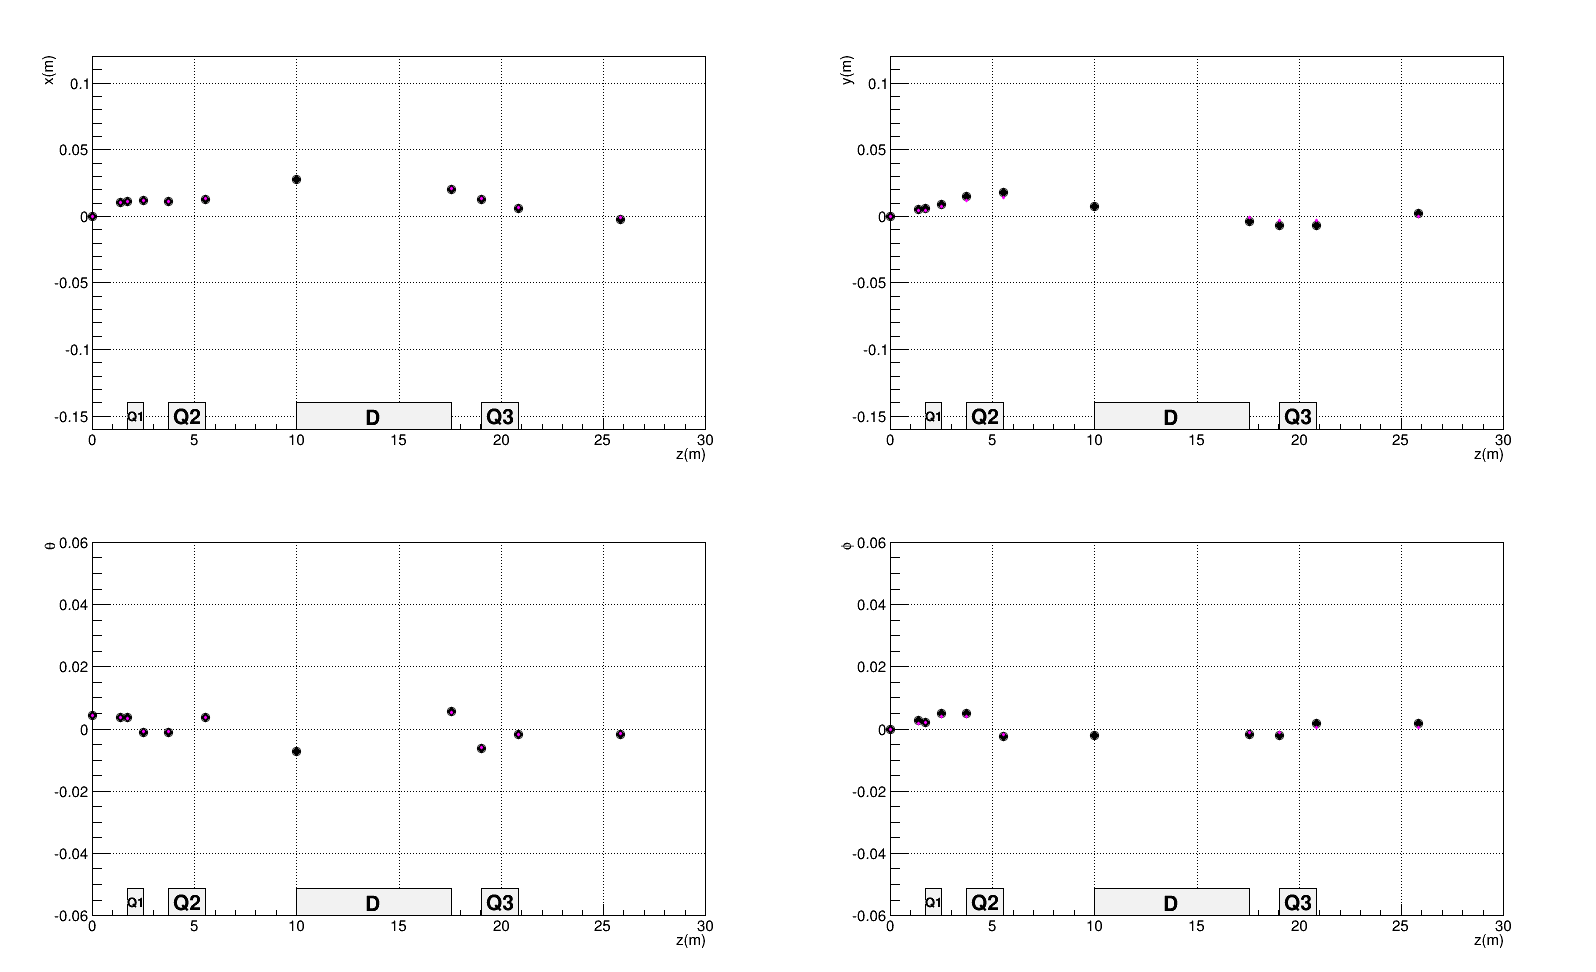
\includegraphics[width=0.95\textwidth]{plots/pres_matrix_t_4.png}
\end{center}
\caption{The results of sending an electron through the HRS with initial target variable $\theta=0.25\text{ degrees}$, and all other variables 0. In the upper left, transport $x$, in the upper right, transport $y$, in the lower left, transport $\theta$, and in the lower right, tranport $\phi$, all as a function of z. The large black points are the results of G4MC. The smaller, superimposed magenta points are the results of SNAKE.}
\end{figure}

\begin{figure}
\begin{center}
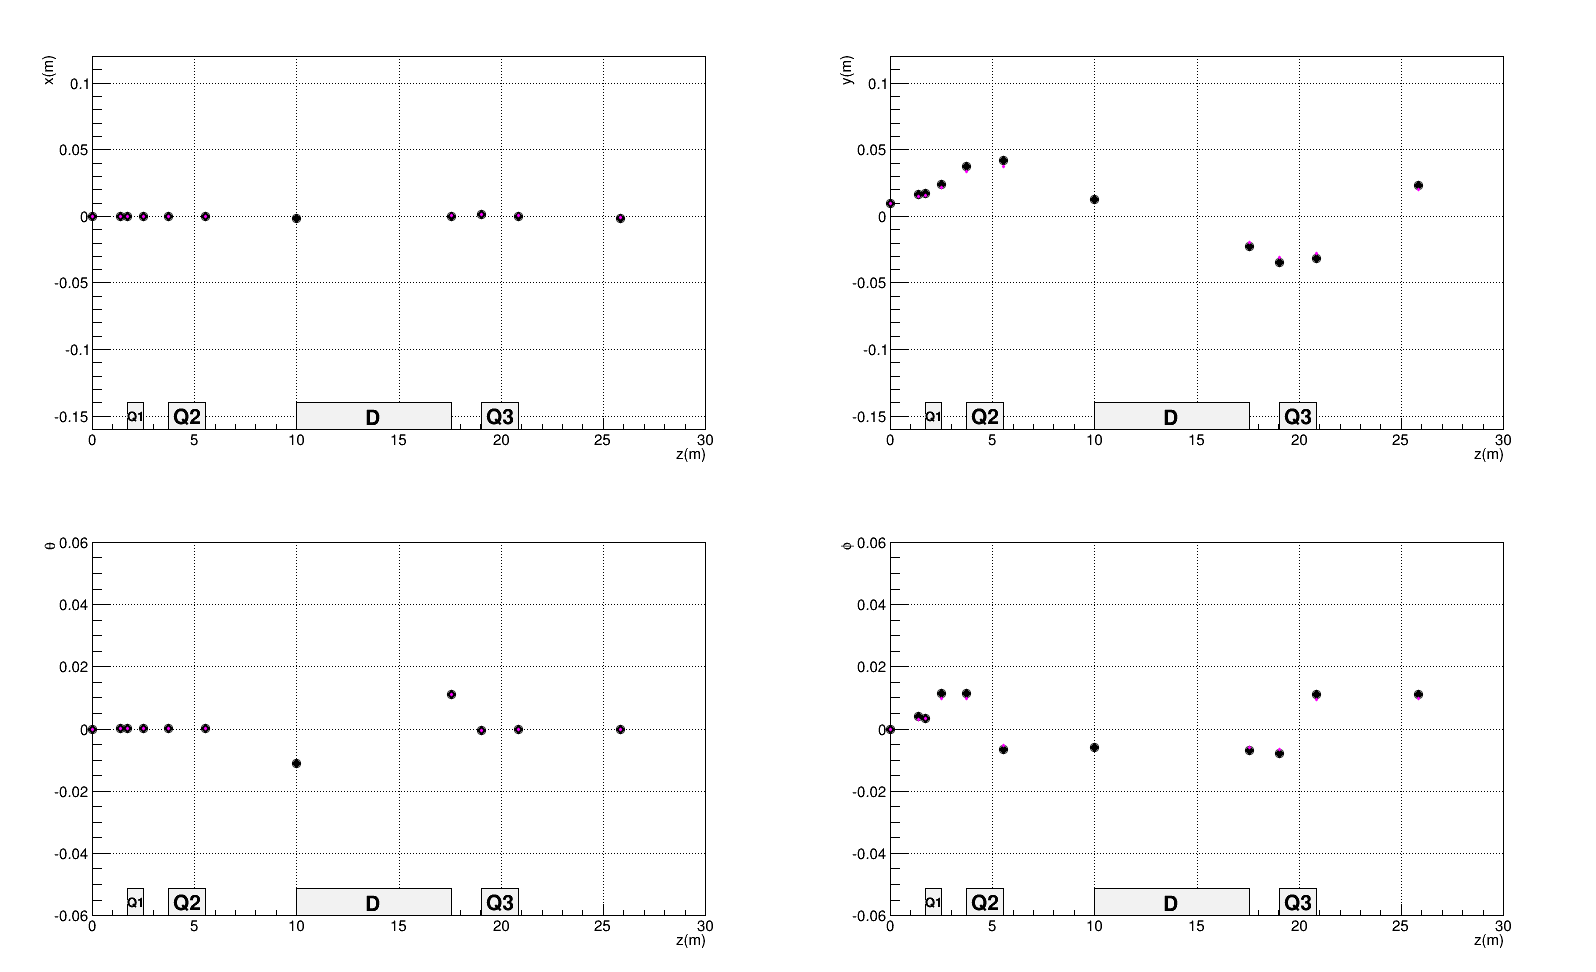
\includegraphics[width=0.95\textwidth]{plots/pres_matrix_y_4.png}
\end{center}
\caption{The results of sending an electron through the HRS with initial target variable $y=1\text{ cm}$, and all other variables 0. In the upper left, transport $x$, in the upper right, transport $y$, in the lower left, transport $\theta$, and in the lower right, tranport $\phi$, all as a function of z. The large black points are the results of G4MC. The smaller, superimposed magenta points are the results of SNAKE.}
\end{figure}

\begin{figure}
\begin{center}
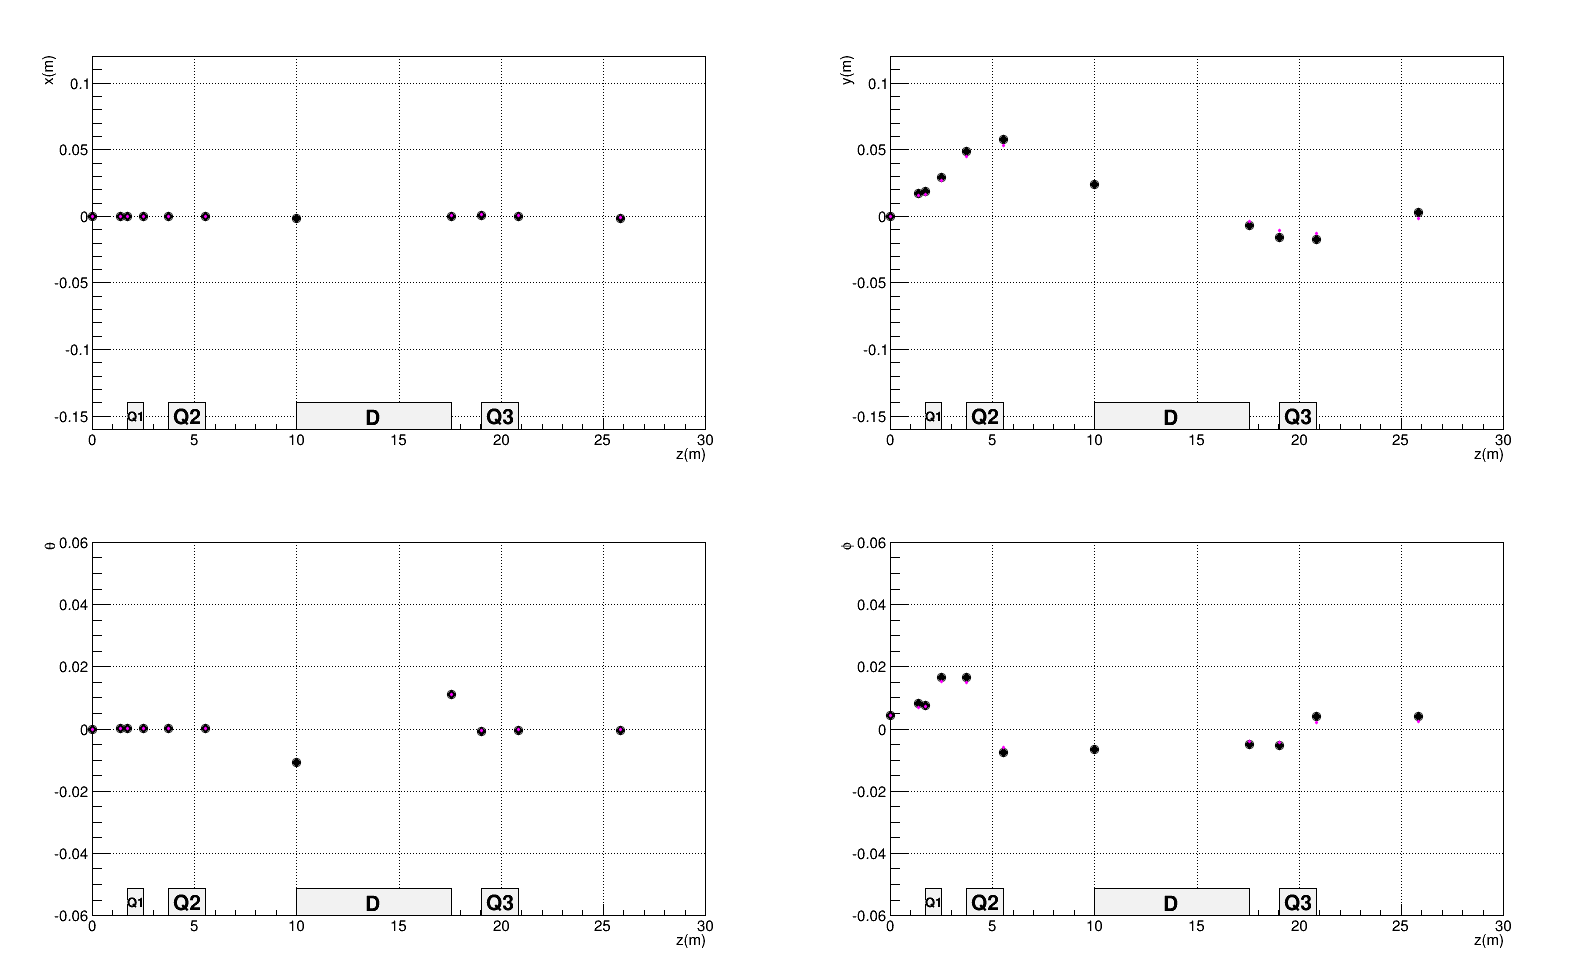
\includegraphics[width=0.95\textwidth]{plots/pres_matrix_p_4.png}
\end{center}
\caption{The results of sending an electron through the HRS with initial target variable $\phi=0.25\text{ degrees}$, and all other variables 0. In the upper left, transport $x$, in the upper right, transport $y$, in the lower left, transport $\theta$, and in the lower right, tranport $\phi$, all as a function of z. The large black points are the results of G4MC. The smaller, superimposed magenta points are the results of SNAKE.}
\end{figure}

\begin{figure}
\begin{center}
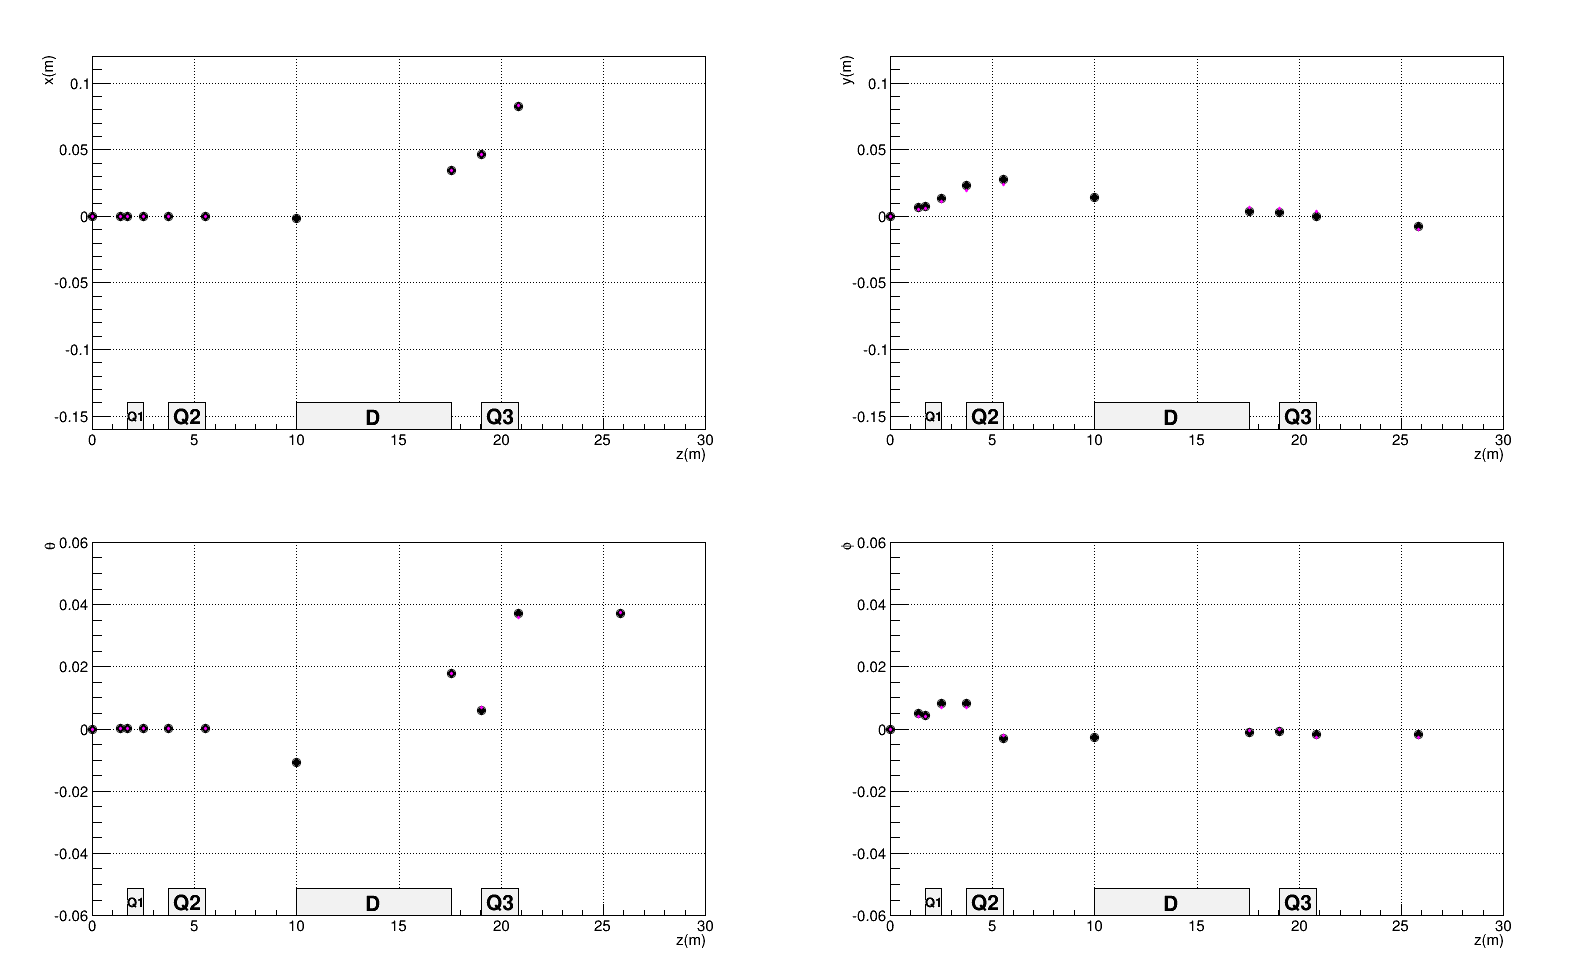
\includegraphics[width=0.95\textwidth]{plots/pres_matrix_d_4.png}
\end{center}
\caption{The results of sending an electron through the HRS with initial target variable $\delta=0.015\text{ degrees}$, and all other variables 0. The central trajectory through the HRS. In the upper left, transport $x$, in the upper right, transport $y$, in the lower left, transport $\theta$, and in the lower right, tranport $\phi$, all as a function of z. The large black points are the results of G4MC. The smaller, superimposed magenta points are the results of SNAKE.}
\end{figure}
\FloatBarrier

\subsection{Reproduction of Data Results}

More important than reproducing the features of legacy MC with G4MC, is to reproduce what is observed in data. We present here a comparison between PREX I data with diamond-lead-diamond target, and G4MC simulation results. The key features to reproduce are: a correct cross section model with radiative corrections and identical distributions at the focal plane. The radiative corrections can be gauged by comparing the $x$ and $\delta$ variables at the focal plane, particularly by looking at the falloff of the radiative tail. The cross section can be compared by looking at $\phi$, which is roughly the lab scattering angle. We note that comparison is quite good, and that radiative effects are fairly well reproduced.

\FloatBarrier
\begin{figure}
\begin{center}
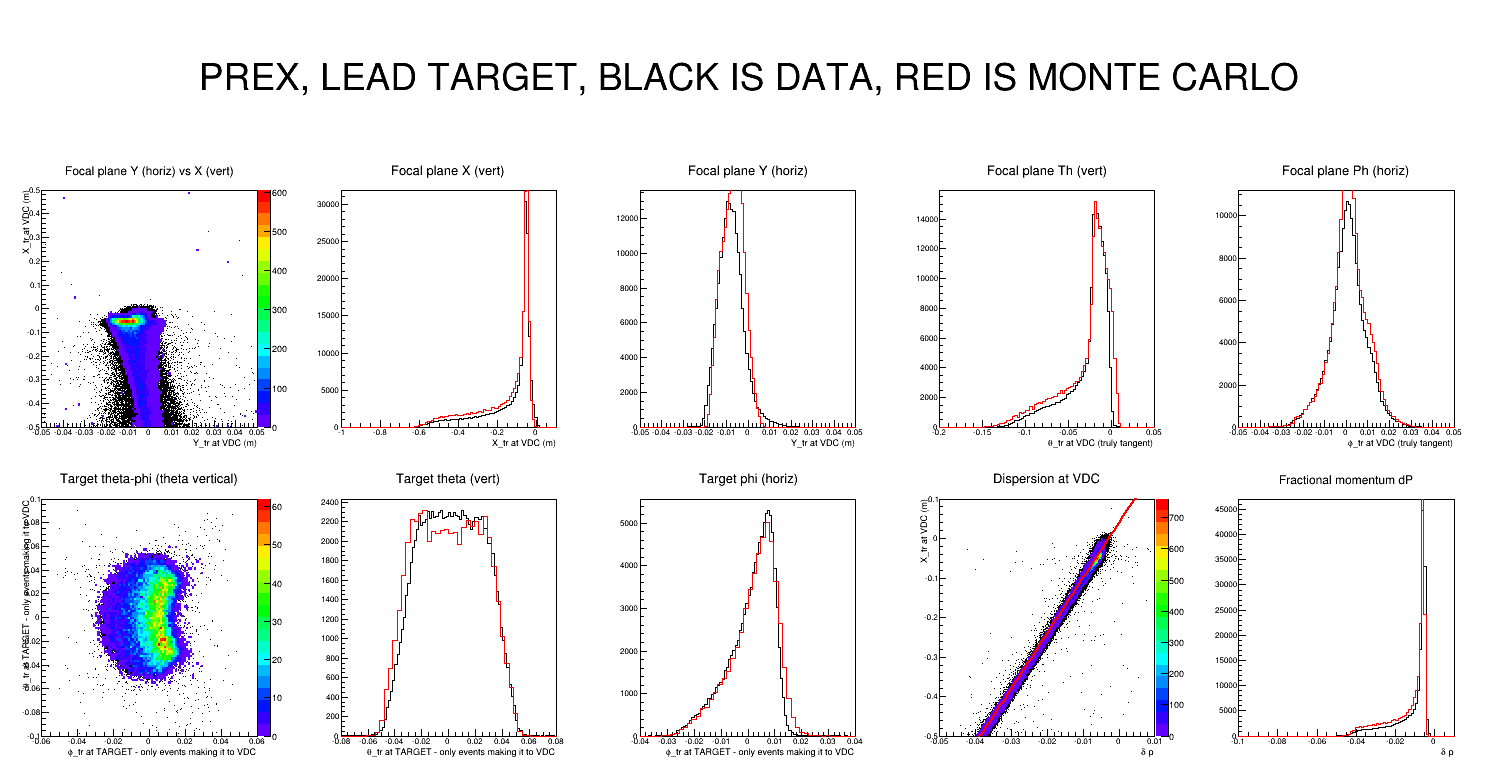
\includegraphics[width=0.95\textwidth]{plots/compare_PREX_noscrape_truerad_tune.png}
\end{center}
\caption{A comparison of data and G4MC, for PREX I, with lead target. Monte Carlo is in red (or color plot), and data is in black (or black scatter plot). The top row shows: $x$ versus $y$ at the focal plane, $x$ at the focal plane, $y$ at the focal plane, $\theta$ at the focal plane, and $\phi$ at the focal plane. The first the plots on the bottom row show: $\theta$ versus $\phi$ at the target, $\theta$ at the target, and $\phi$ at the target. The last two plots on the bottom row show: the dispersion relation ($x$ at the focal plane as a function of $\delta$), and $\delta$ }
\end{figure}
\FloatBarrier

\newpage
\section{Application of G4MC}

\subsection{ Acceptance }

The Q1 quads that were used for PREX I will be replaced with warm Short Orbit Spectrometer (SOS) quads from PREX II and CREX. These quads have a smaller aperture, and a different length. The SOS quad has a radius of 12.827 cm compared to the 15.0 cm radius of the old quad. Due to the decreased aperture size, we expect a reduction in acceptance. We present here a set a plots which quantifies that loss of acceptance at just below 4\%.

\FloatBarrier
\begin{figure}
  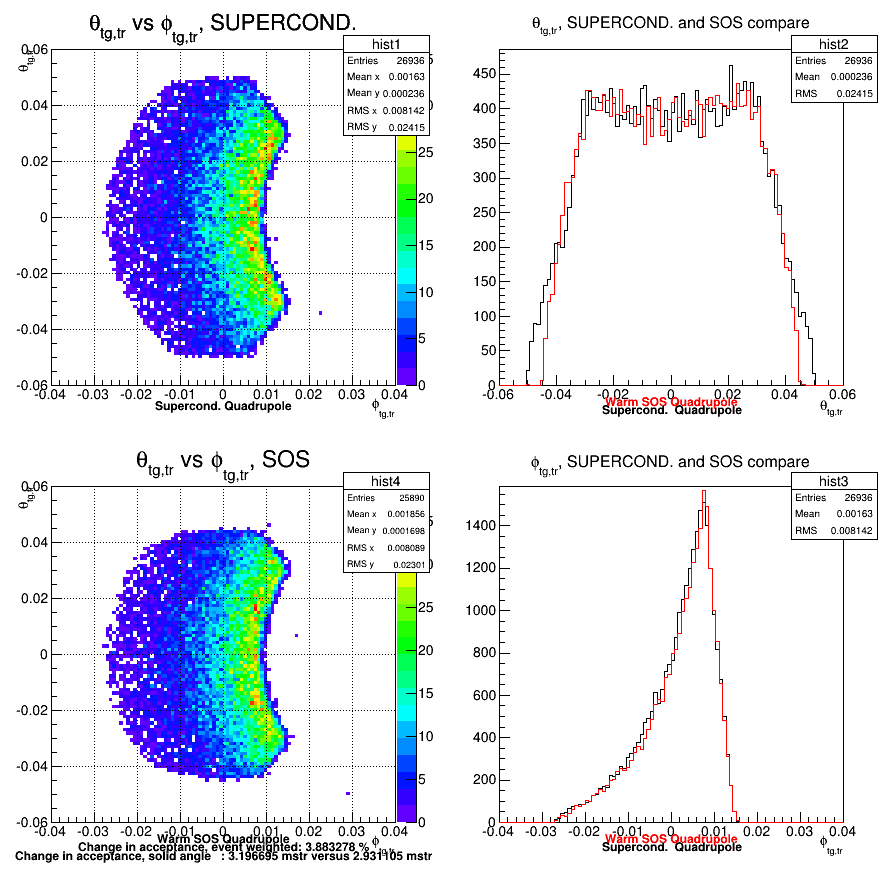
\includegraphics[width=0.95\textwidth]{plots/acc.png}
  \caption{On the upper left, $\theta$ versus $\phi$ in transport coordinates for the old superconducting quadrupole. On the lower left, $\theta$ versus $\phi$ in transport coordinates for the warm SOS quadrupole. In the upper right, $\theta$ for both SOS (red) and superconducting (black) quads. In the lower right, $\phi$ for both SOS (red) and superconducting (black) quads.}
\end{figure}
\FloatBarrier

The acceptance was also benchmarked against the results of HAMC.

\FloatBarrier
\begin{figure}
  \includegraphics[width=0.95\textwidth]{plots/crex_col0.png}
  \caption{The acceptance, HAMC in black points, and G4MC in green points. The comparison shows that both simulations produce the same acceptance.}
\end{figure}
\FloatBarrier

\subsection{ Figure of Merit }

A figure of merit for PREX II and CREX will justify the optimal energy and angles to run at. We present here the figure of merit as a function of energy for a fixed angle of $5^\circ$ for PREX, and $6^\circ$ for CREX. The results for PREX I and PREX II are similar, but as expected, PREX II is somewhat lower due to the loss of acceptance from the SOS quad. The difference, however is small, and justifies being able to run PREX II and CREX with the decreased acceptance.

\FloatBarrier
\begin{figure}
  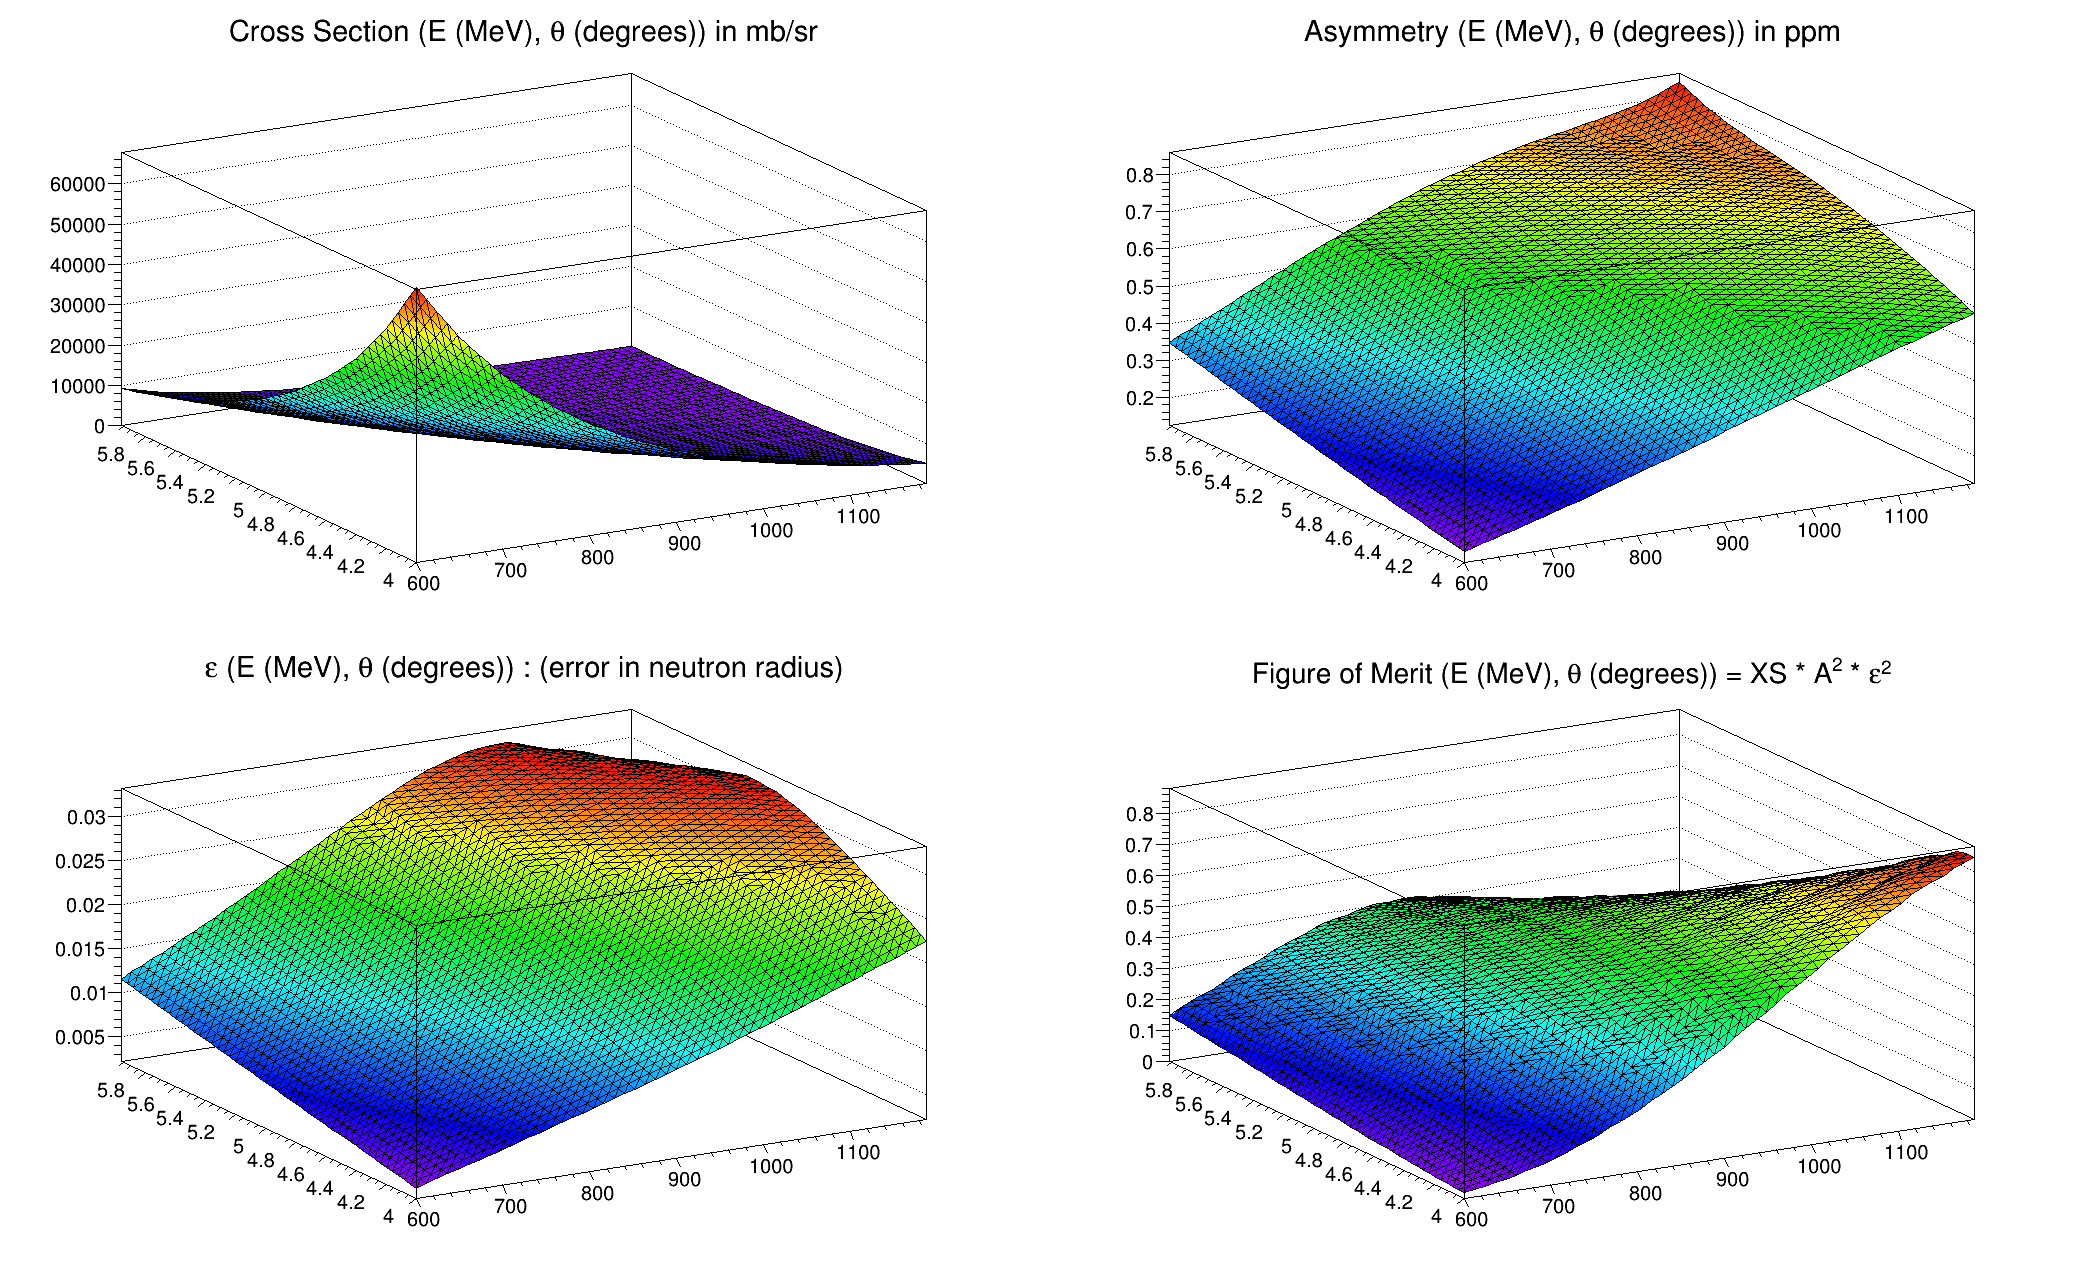
\includegraphics[width=0.95\textwidth]{plots/contour_p.png}
  \caption{PREX: Horowitz generated cross sections, asymmetries, neutron radius fractional error, and FOM as a function of energy and angle}
\end{figure}

\begin{figure}
  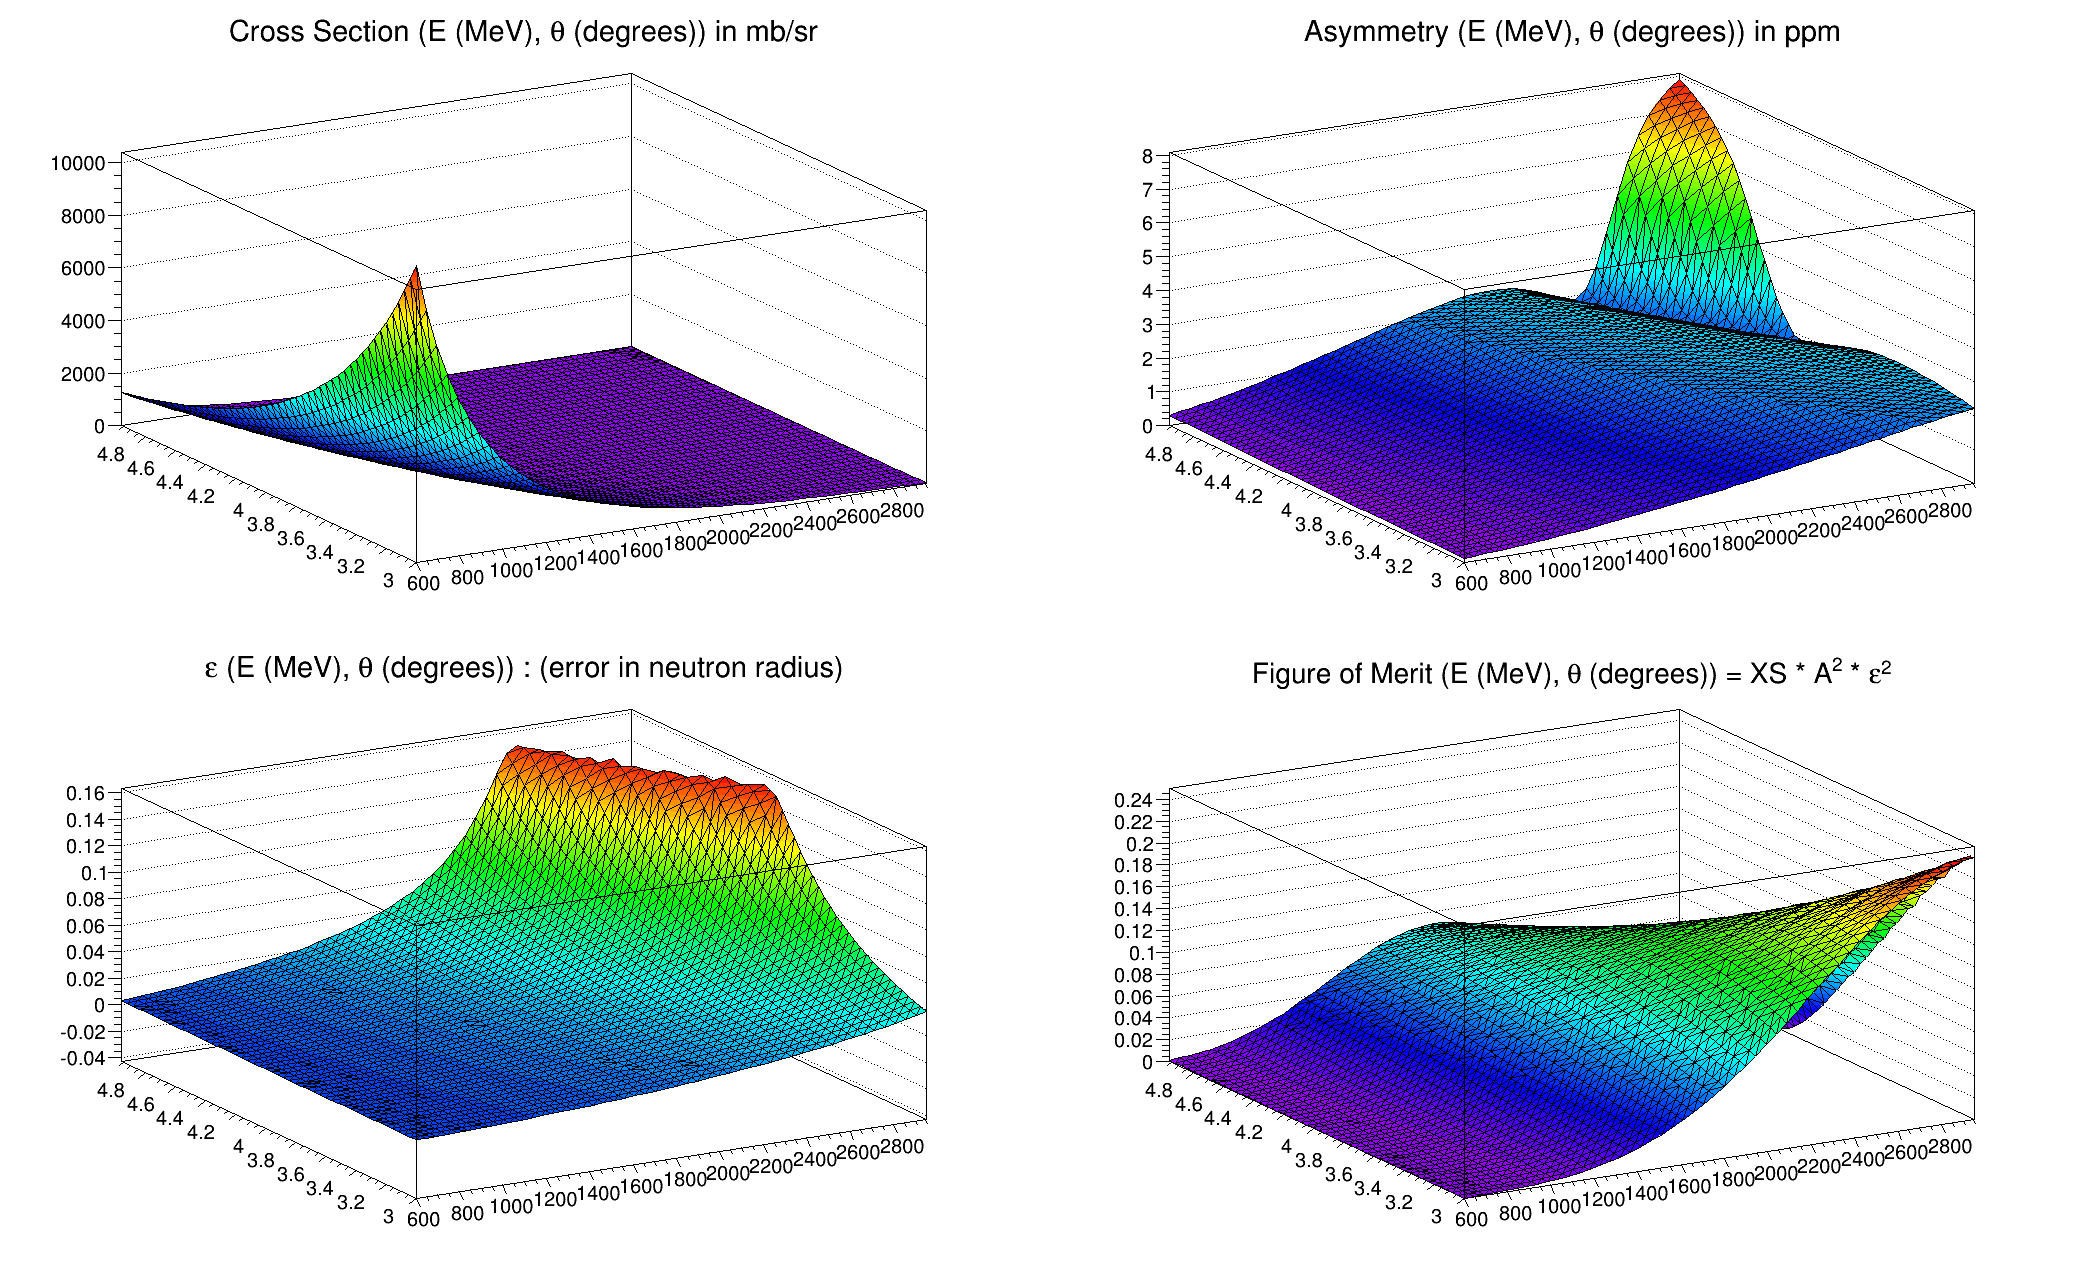
\includegraphics[width=0.95\textwidth]{plots/contour_c.png}
  \caption{CREX: Horowitz generated cross sections, asymmetries, neutron radius fractional error, and FOM as a function of energy and angle}
\end{figure}

\begin{figure}
  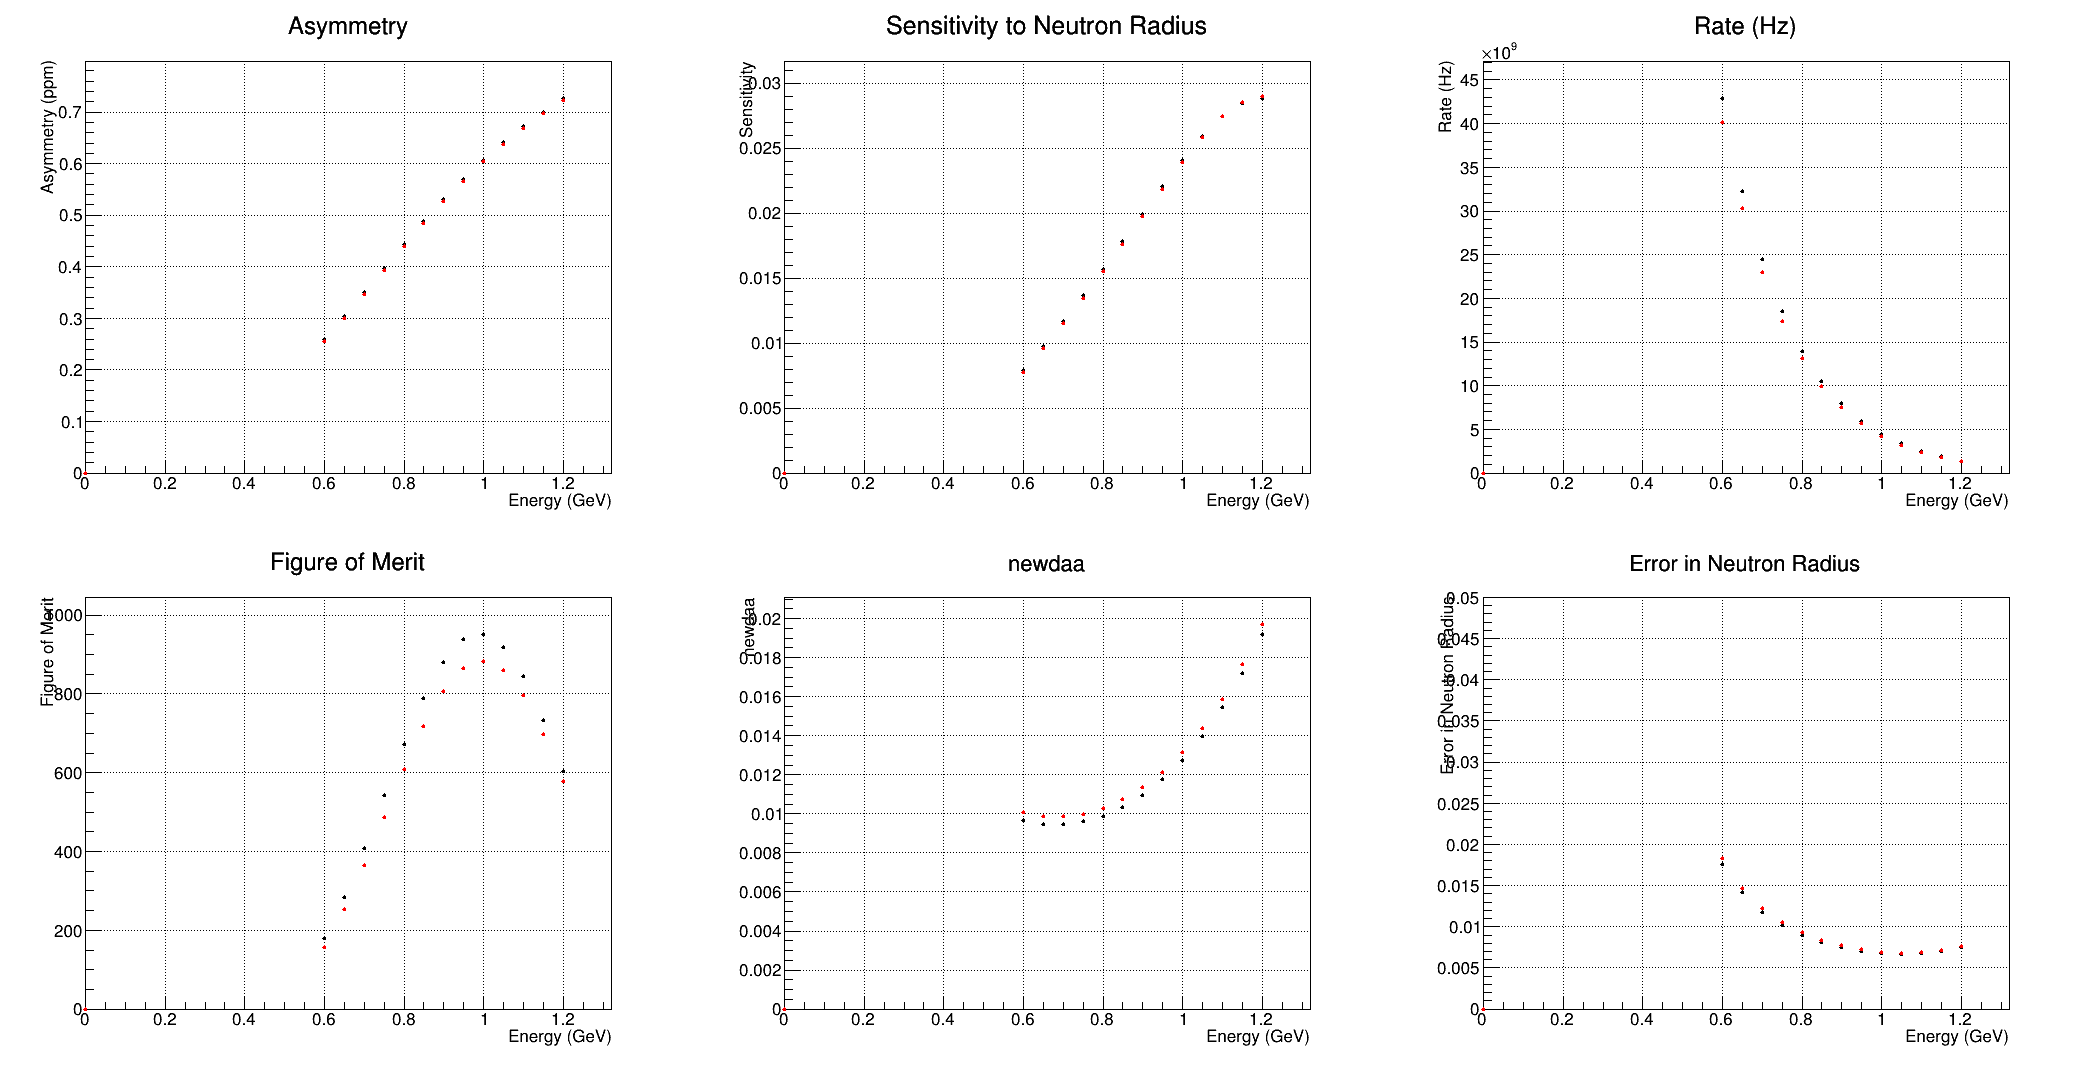
\includegraphics[width=0.95\textwidth]{plots/fom_p.png}
  \caption{Figure of Merit (FOM) for PREX I (black) and PREX II (red). One observes the slight loss of FOM due to the loss of acceptance from the SOS quad.}
\end{figure}

\begin{figure}
  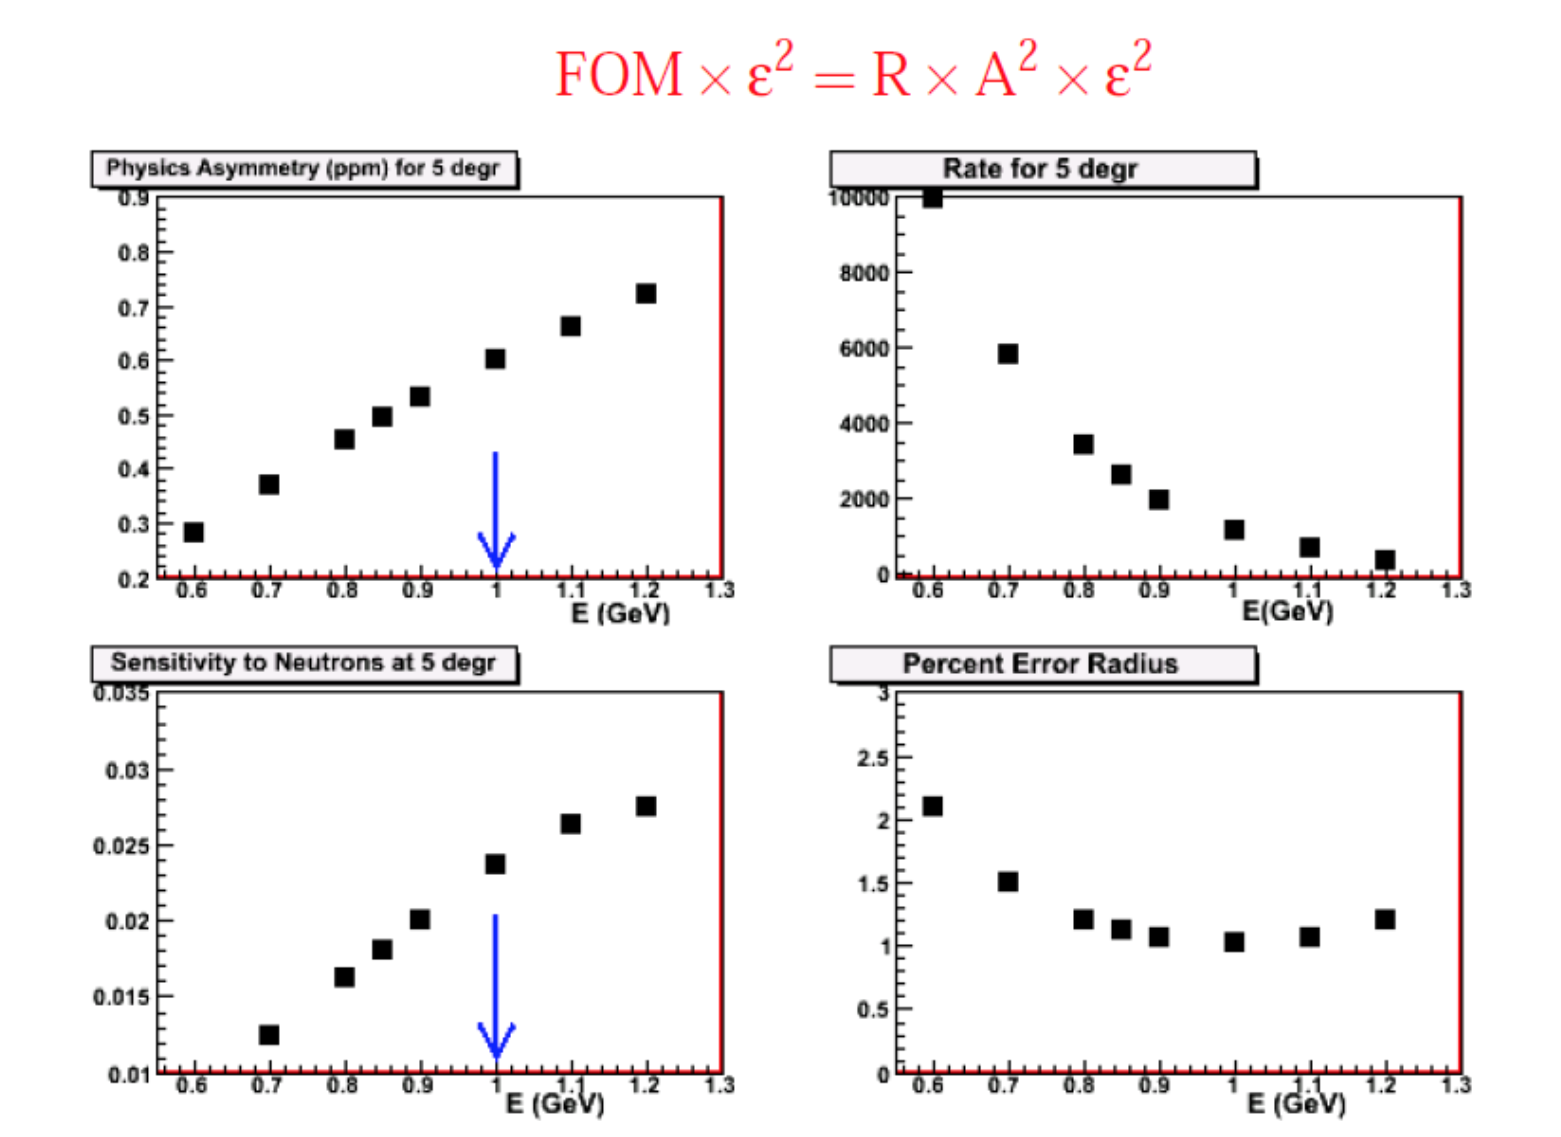
\includegraphics[width=0.95\textwidth]{plots/fom_old.png}
  \caption{Old Figure of Merit (FOM) for PREX I HAMC study}
\end{figure}

%\begin{figure}
%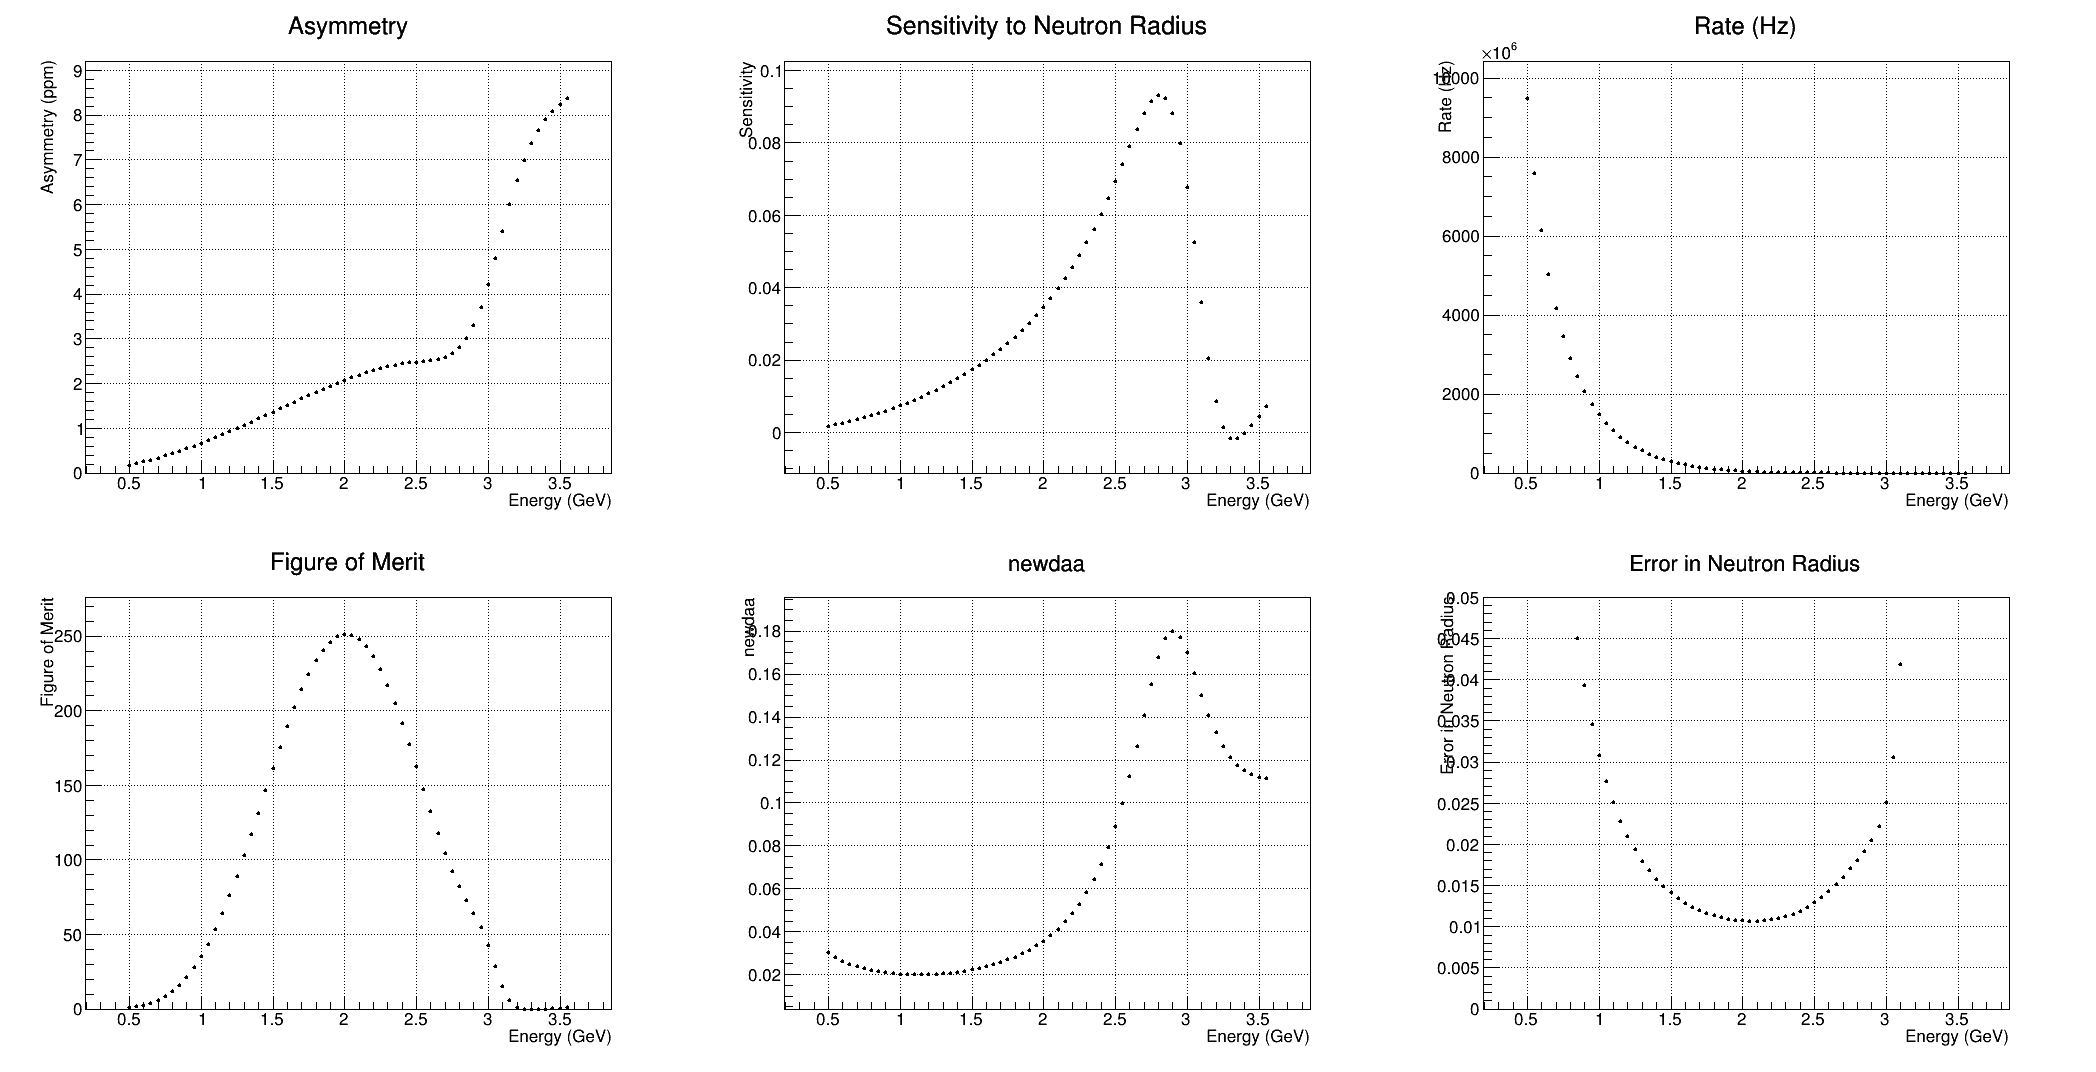
\includegraphics[width=0.95\textwidth]{plots/fom_c.png}
%\caption{Figure of Merit (FOM) for CREX.}
%\end{figure}
\FloatBarrier

The possibility arose of running CREX at 5 degrees back to back with PREX at 5 degrees, instead of CREX at 4 degrees and PREX at 5 degrees. An analysis was performed, using G4MC, to look at the possibility of this configuration change, most importantly looking at the figure of merit. The conclustion was that, while 5 degrees CREX gives a slightly less advantageous figure of merit, that the loss is marginal.

\FloatBarrier

\begin{figure}
\includegraphics[width=0.95\textwidth]{plots/4degcrex.png}
\caption{Figure of Merit (FOM) for CREX at 4 degrees.}
\end{figure}

\begin{figure}
\includegraphics[width=0.95\textwidth]{plots/5degcrex.png}
\caption{Figure of Merit (FOM) for CREX at 5 degrees.}
\end{figure}

\FloatBarrier

\subsection{ Resolution }

The resolution of the HRS spectrometers when moving from PREX to PREX II (superconducting Q1 to SOS Q1) can be quantified by looking at the width of focal plane distribution in  $x$. Here, we take the full-witdh-half-maximum as the measure of resolution. We show here that the resolution is only slighly worsened by moving to the SOS Q1.

\FloatBarrier
\begin{figure}
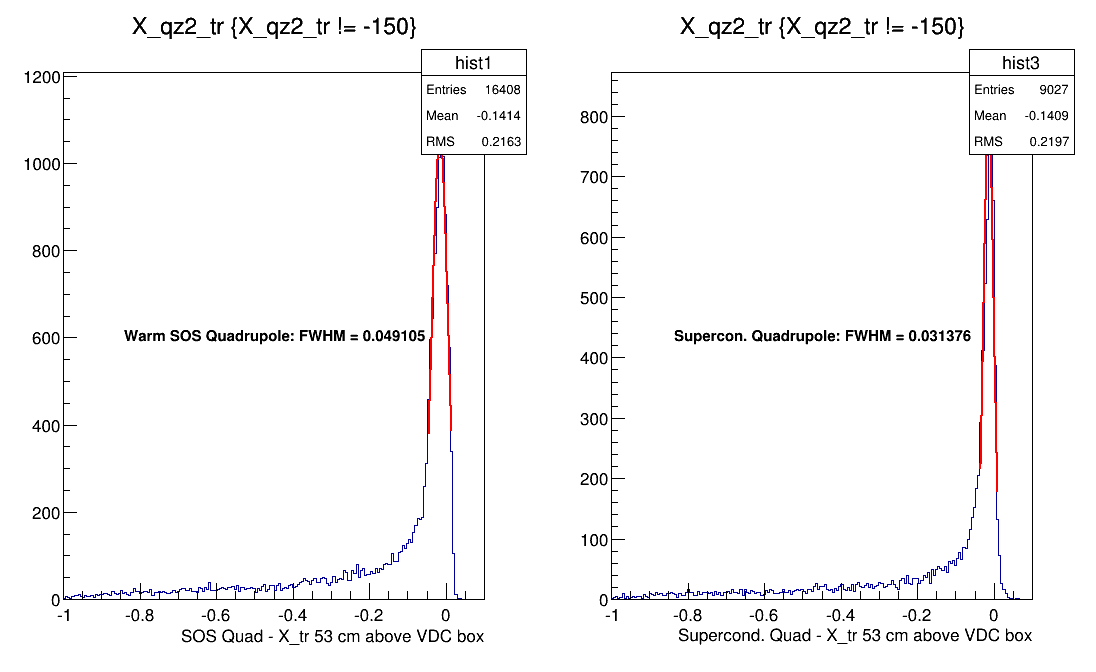
\includegraphics[width=0.95\textwidth]{plots/res.png}
\caption{Resolution}
\end{figure}
\FloatBarrier

\subsection{ Q1 Collimators }

In PREX I, one of the criteria that we imposed on the collimator in front of Q1 was that it completely define the acceptance for the experiment. Since the bore radius of the SOS Q1 for PREX II and CREX is smaller than the superconducting Q1 from PREX I, the old collimator design will not be sufficient to completely define the acceptance. In this case, we are motivated to redesign the collimator to ensure that the acceptance is still completely defined by the new collimator. We present here a possible design for the new collimator which would completely define the acceptance for both the CREX and PREX II experiments.

\FloatBarrier
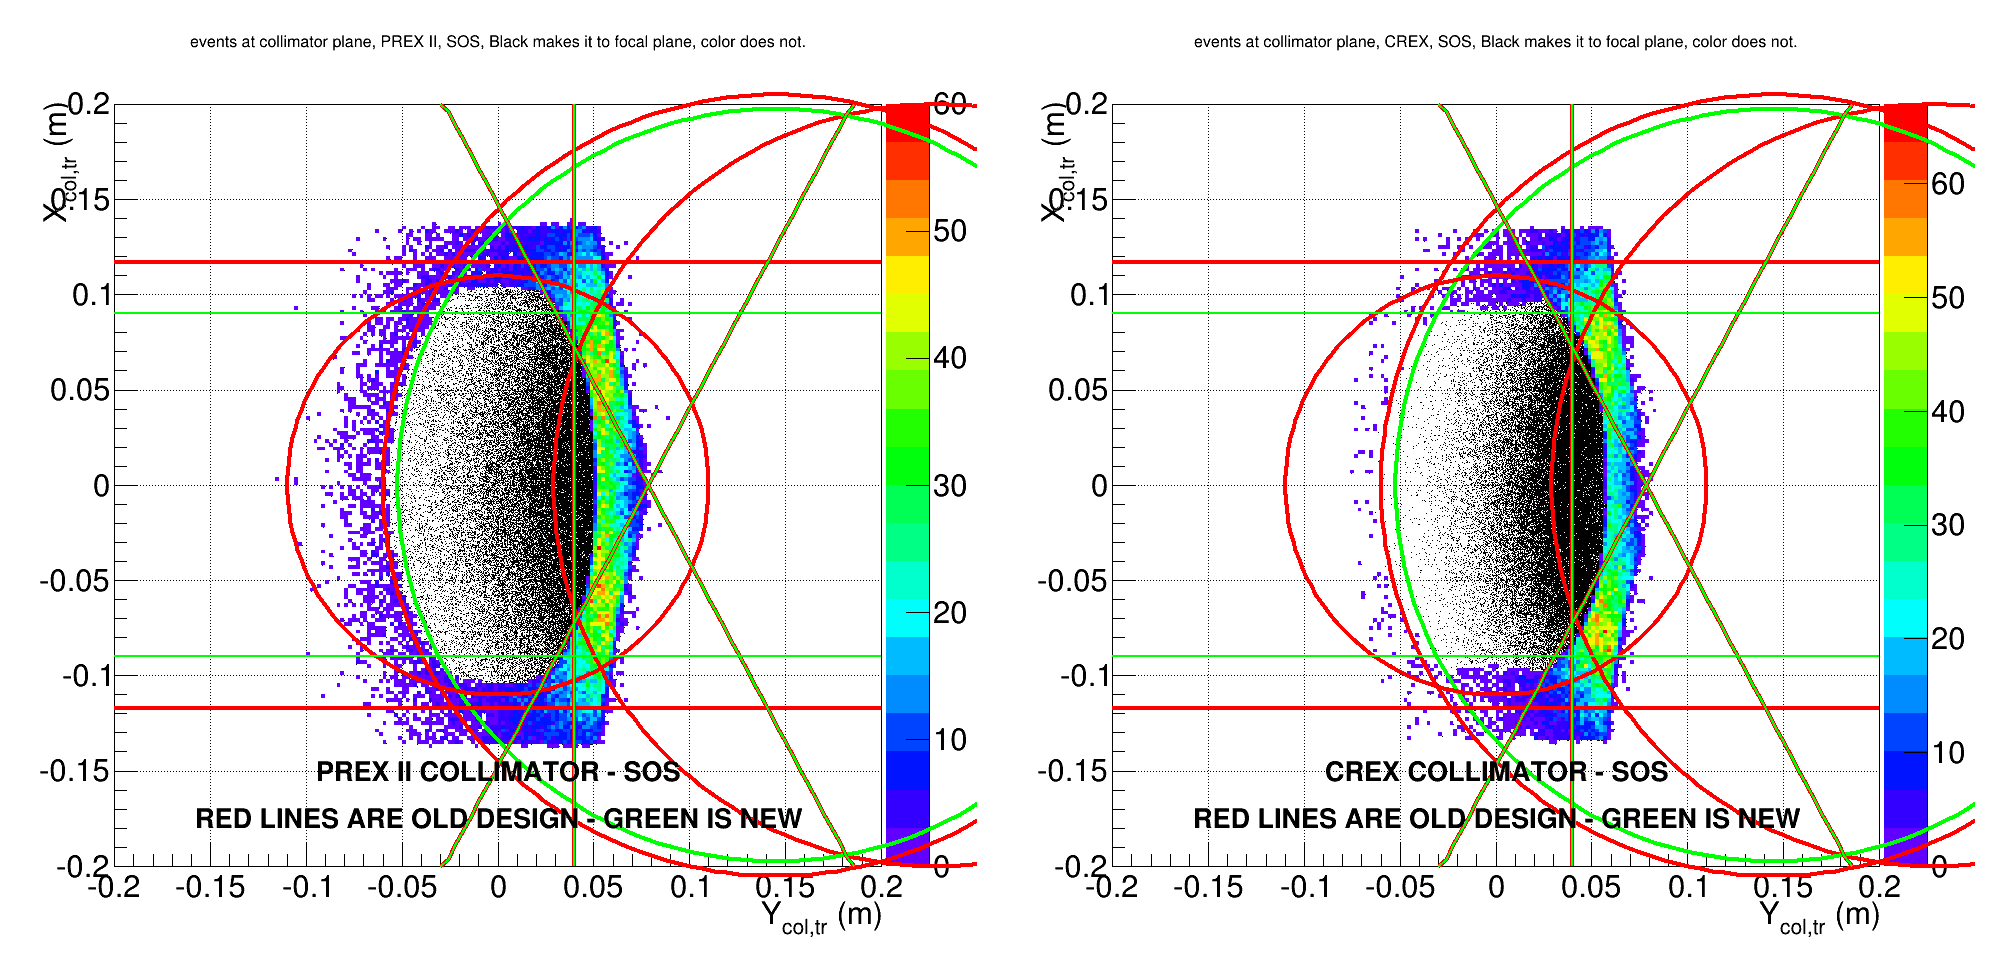
\includegraphics[width=0.95\textwidth]{plots/newcol.png}
\FloatBarrier

\subsection{ ``Keep-out'' Regions }

In order to guarantee that the acceptance is truly defined by our collimator, we must present the engineers with volumes which cannot be obstructed by any mechanical objects. We accomplished this by looking at events crossing the planes at the septum entrance, the septum midplane, the septum exit, and the Q1 entrance. We took all events which eventually reach the quartz at each such plane, and defined areas which completely contained those particles. The color plot represents particles which eventually reach the quartz detector. The black lines define our keep-out zones. The volume is then determined by fitting functions to the corners of these four boxes. The engineers then agree not to place anything within that zone.

\FloatBarrier
%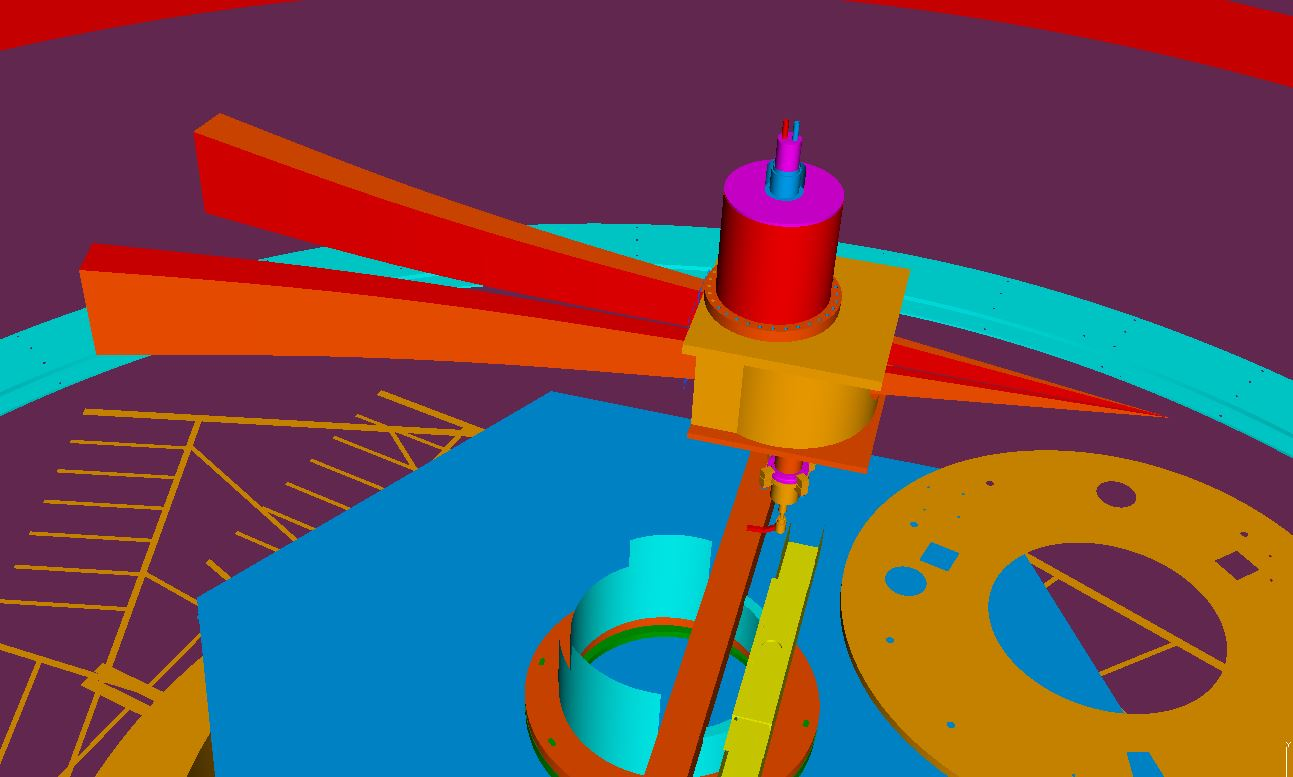
\includegraphics[width=0.95\textwidth]{plots/image1.JPG}

%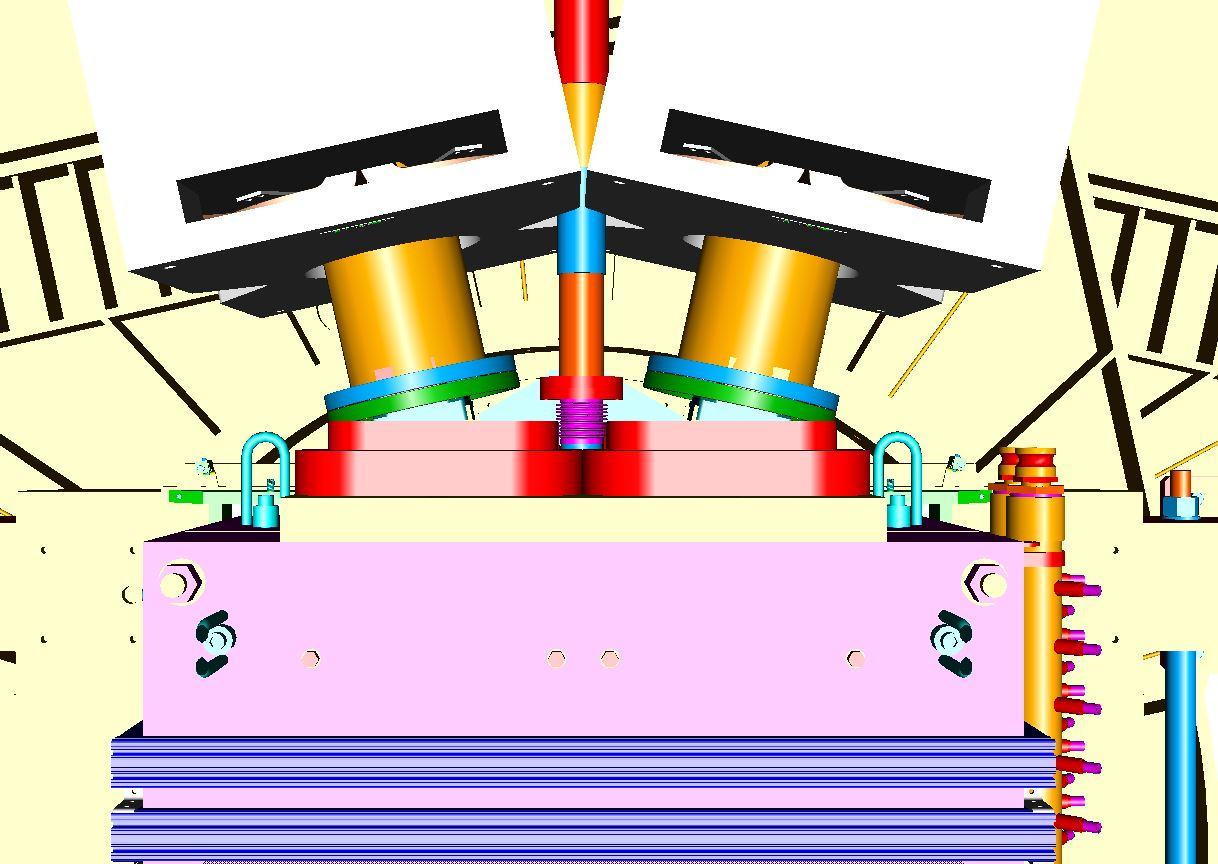
\includegraphics[width=0.95\textwidth]{plots/image2.JPG}
\begin{figure}
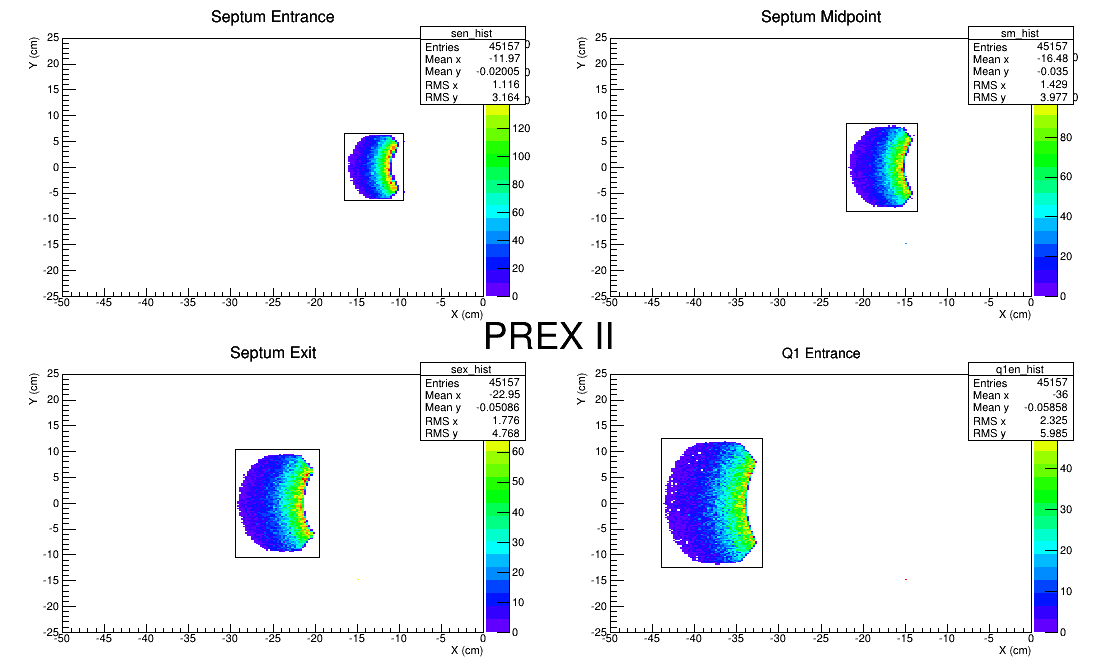
\includegraphics[width=0.95\textwidth]{plots/keepout.png}
\caption{Keep-out zones for PREX II, at the septum entrance, the septum midplane, the septum exit, and the Q1 entrance. The color plot represents particles which eventually reach the quartz detector. The black lines define our keep-out zones.}
\end{figure}

\begin{figure}
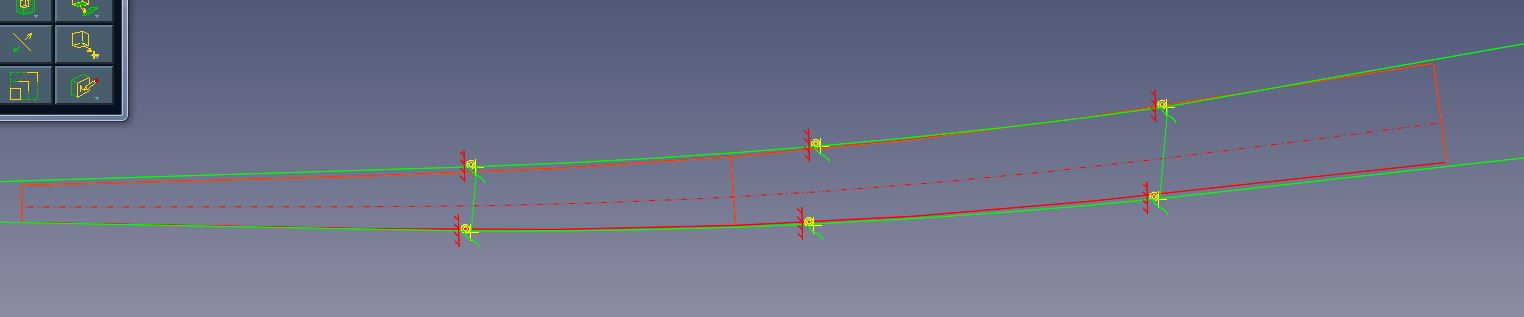
\includegraphics[width=0.95\textwidth]{plots/PREXvsPREXII.JPG}
\caption{A visual comparison of PREX I and PREX II keep-out zones. PREX I is in green and PREX II is in red. The comparison shows that the keep-out zone, as expected, did not change much.}
\end{figure}

\FloatBarrier

\subsection{ Focal Plane Distributions - CREX}

In order to finalize the design of the CREX quartz pieces, the distributions at the focal plane have to be determined. The width of the distributions have to be completely contained by the quartz detectors. For CREX, we have taken the assumption that we will place the quartz detector at 40 cm vertical to the top of the VDC. The quartz will be perpendicular to the nominal trajectory. 

\FloatBarrier
\begin{figure}
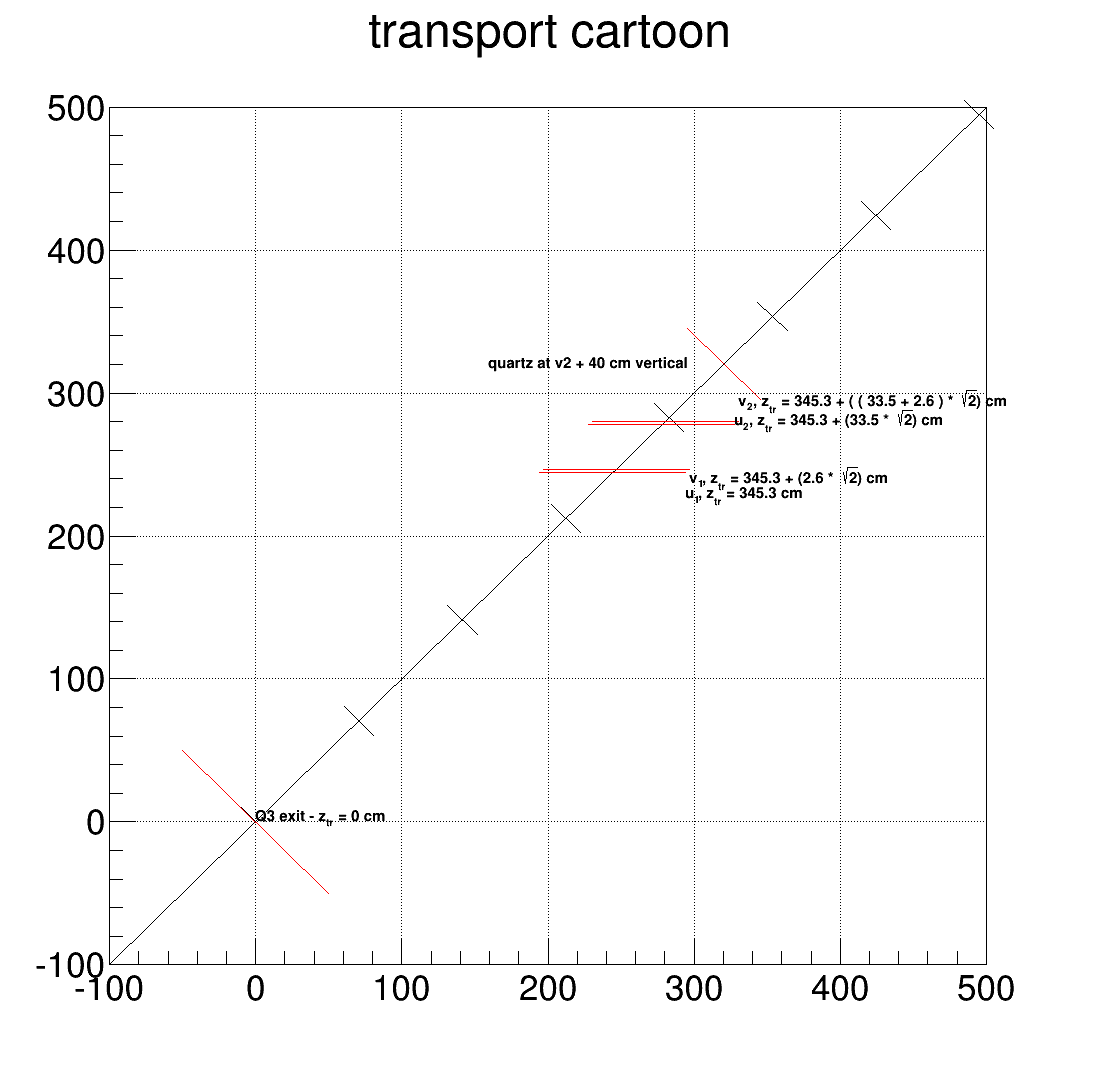
\includegraphics[width=0.95\textwidth]{plots/transportcartoon.png}
\caption{A cartoon describing the geometry of the quartz setup relative to the Q3 and VDCs}
\end{figure}

\begin{figure}
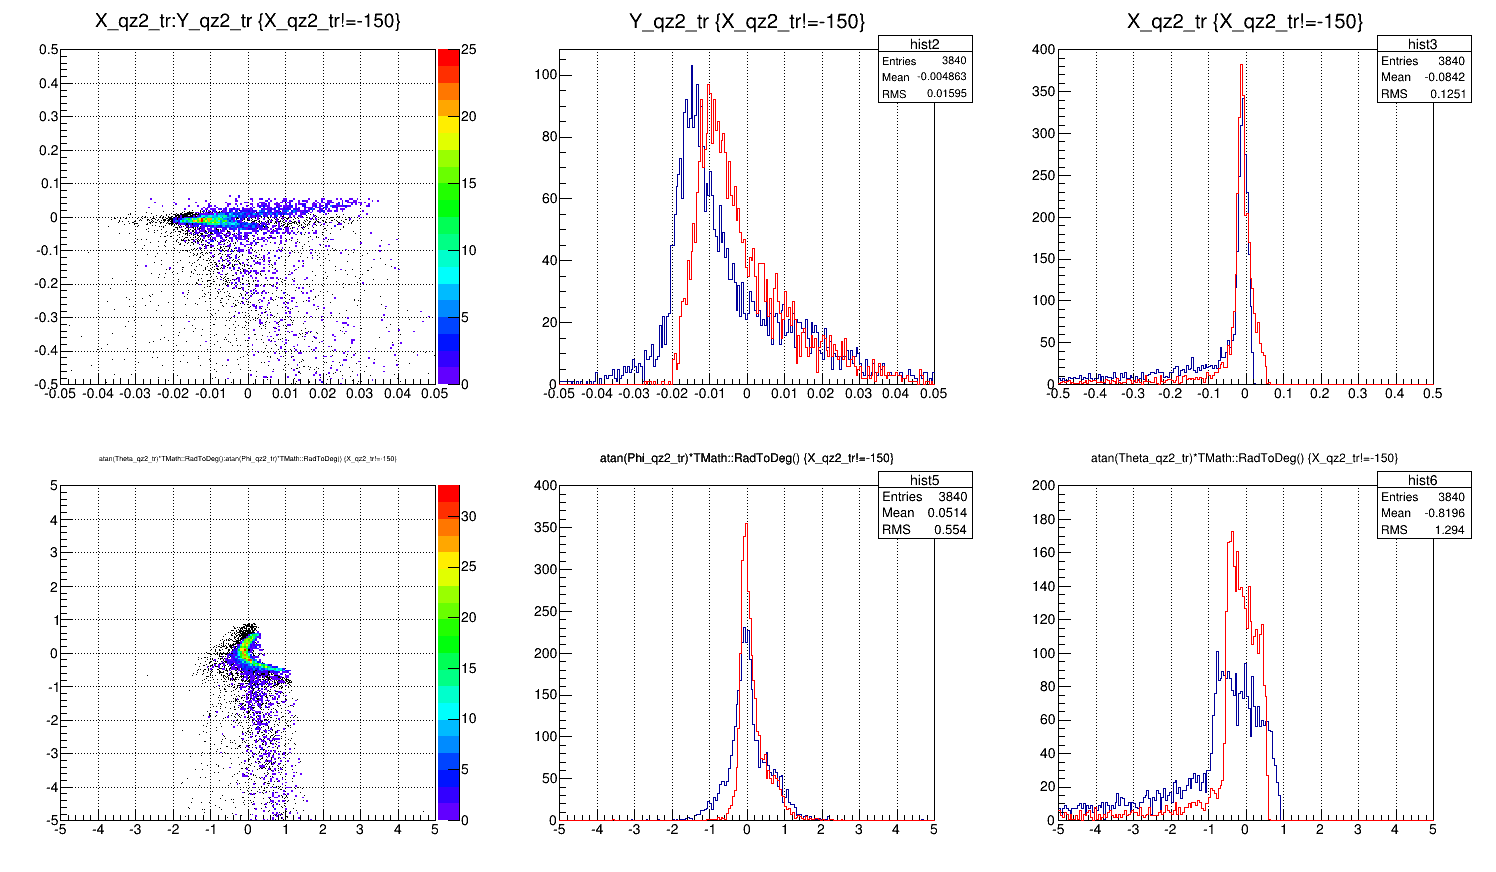
\includegraphics[width=0.95\textwidth]{plots/crex_footprint.png}
\caption{On top, the position distributions at the quartz detector, on bottom, the angular distributions. PREX I is in blue lines (or black scatter) and CREX is in red lines (or color scatter)}
\end{figure}

\FloatBarrier

\subsection{ CREX Tune }

A preliminary tune has been developed for CREX. The final optimization of this tune needs to be completed.

\subsection{ Poletip Scattering}

Iron in the yokes of the magnets has the tendency to have its electrons ploarized. One existing concern is that if there is significant scraping of electrons in the dipole that M\o ller scattering could occur with those polarized electrons as the target electron, leading to a false asymmetry in the detector. Studying the degree to which this is or is not a problem is possible with this simulation. 

\newpage
\section{Outlook and Possible Refinements}

This project is maintained by Nickie, \href{mailto:nicholas@hirlinger-saylor.com}{nicholas@hirlinger-saylor.com}

\section{Running the Code}

When beginning a project, create a folder inside the main directory. Run G4MC inside the created directory with the following files:

\begin{itemize}
\item Input files:
  \begin{itemize}
  \item HRSUsage.ini
  \item BField\_Septum.ini
  \item Detector.ini
  \item Detector\_CREX.ini
  \end{itemize}
\item Cross section tables (Horowitz, Zidu)
  \begin{itemize}
  \item ca48\_fsu.dat
  \item ca48\_fsu\_stretched.dat
  \end{itemize}
\item septum field maps
  \begin{itemize}
  \item prex\_septumfield.jixie.dat
  \item CREX\_juliette.dat
  \item PREX\_juliette.dat
  \end{itemize}
\item database
  \begin{itemize}
  \item db\_L.vdc.dat
  \item db\_R.vdc.dat
  \end{itemize}
\item macros
  \begin{itemize}
  \item gui.mac
  \item beam.mac
  \end{itemize}
\end{itemize}

All parameters in these files remain fixed as there currently are presented in the repository, except the following changes in the table:

\begin{tabular}{| l | l | l | l |}
\hline
\textbf{File} & \textbf{Parameter} & \textbf{PREX} & \textbf{CREX}\\
\hline
HRSUsage.ini & SnakeModel & 49 & 53 \\
\hline
&SeptumFieldMap & PREX\_juliette.dat & CREX\_juliette.dat \\
\hline
& BeamEnergy & 1063 & 2200 \\
\hline
& LHRSMomentum & 1063 & 2200 \\
\hline
& RHRSMomentum & 1063 & 2200 \\
\hline
\hline
BField\_Septum.ini & Septum\_DefaultMomentumL & 1.063 & 2.32 \\
\hline
 & Septum\_DefaultMomentumR & 1.063 & 2.32 \\
\hline
\hline
Detector\_CREX.ini & TargetZOffset & -1053.79 & -1520 \\
\hline
&TargetL& 0.5& 5.9\\
\hline
&SetupPREXTarget& 1& 0\\
\hline
&SetupCREXTarget& 0& 1\\
\hline
&RSeptumAngle& 355.0& 356.0\\
\hline
&LSeptumAngle& 5.0& 4.0\\
\hline
\hline
beam.mac& /mydet/gunZHigh& -1053.54& -1517.05\\
\hline
&/mydet/gunZLow& -1054.04& -1522.95\\
\hline
&/mydet/particle1/momentum& 1.063 GeV& 2.2 GeV\\
\hline
&/mydet/particle1/thetaLow &4 deg& 3 deg\\
\hline
&/mydet/particle1/thetaHigh &7 deg& 6 deg\\
\hline
&/mydet/particle1/phiLow &140 deg &90 deg\\
\hline
&/mydet/particle1/phiHigh &220 deg &270 deg\\
\hline
\end{tabular}
\\
In BField\_Septum.ini, one has to make sure the number of steps, and steps size of the field map is indicated. Automation of this is desireable.\\
\\
\\
Batch: G4MC -m 1 ./beam.mac\\
\\
Interactive: G4MC -i -x 1\\
\\
Advantages: Input files can be used to make quick configuration changes without recompiling.\\
\\
Disavantages:\\
\\
Magnets have to be retuned in the code.\\
\\
The number of inputs is overwhelming, despite most of them not changing.\\
\\
\\
My proposed solution is the following:\\
\\
\begin{enumerate}
  \item Develop script which brings user through a menu, where she can select certain experiment settings.
  \item Based on settings requested, the .ini files will be generated automatically, and put in a project folder.
  \item User can then just run ``G4MC -m 1 ./beam.mac'', or the script can run the program automatically.
  \item Allow for ``custom'' tunes by having magnetic fields be another .ini input parameter, if one of the default settings is not desired.
  \item Hardcode items that will never be changed, but are present in the .ini files
  \item 
\end{enumerate}

\section{Output Variables}

In general, the output variables obey the following rules:\\
\\
VARNAME\_PLANENAME(\_tr)\\
\\
VARNAME is the name of the variable, and is usually: $x$, $y$, $\theta$, or $\phi$.\\
\\
PLANENAME is the name of a sensitive detector in the simulation, for example: ``sen'' for septum entrance, and ``q1ex'' for quadrupole 1 exit.\\
\\
The trailing suffix ``\_tr'' indicates that the variable is in TRANSPORT COORDINATES. The absence of the ``\_tr'' suffix indicates that it is in HALL COORDINATES, where the pivot is the origin.\\
\\
Hall coordinates are such that +z is in the direction of the beam, and +y is pointing out of the earth.\\
\\
Transport coordinates are such that +z is in the direction of the central trajectory, and +x is pointing downwards. Additionally, the angles $\theta$ and $\phi$ are actually the tangent of the angles:  \\
\\
$\theta = \frac{x}{z}, \phi = \frac{y}{z}$\\
\\
\begin{longtable}{| l | l | l |}
\hline
\textbf{variable name}   & \textbf{meaning} & \textbf{coordinates} \\
\hline
X0              & X at target &  hall \\
\hline
Y0              & Y at target & hall \\
\hline
Z0              & Z at target & hall \\
\hline
P0              & P at target & hall \\
\hline
Theta0          & $\theta$ at target & hall \\
\hline
Phi0            & $\phi$ at target & hall \\
\hline
X0\_tr           & X at target & transport \\
\hline
Y0\_tr           & Y at target & transport \\
\hline
Z0\_tr           & Z at target & transport \\
\hline
Theta0\_tr       & $\tan{\theta}$ at target & transport \\
\hline
Phi0\_tr         & $\tan{\phi}$ at target & transport \\
\hline
\hline
X\_sen              & X at septum entrance  & hall \\
\hline
Y\_sen              & Y at septum entrance  & hall \\
\hline
Z\_sen              & Z at septum entrance  & hall \\
\hline
P\_sen              & P at septum entrance  & hall \\
\hline
Theta\_sen          & $\theta$ at septum entrance  & hall \\
\hline
Phi\_sen            & $\phi$ at septum entrance  & hall \\
\hline
X\_sen\_tr           & X at septum entrance  & transport\\
\hline
Y\_sen\_tr           & Y at septum entrance  & transport\\
\hline
Z\_sen\_tr           & Z at septum entrance  & transport\\
\hline
Theta\_sen\_tr       & $\tan{\theta}$ at septum entrance  & transport\\
\hline
Phi\_sen\_tr         & $\tan{\phi}$ at septum entrance  & transport\\
\hline
\hline
X\_sm              & X at septum midpoint  & hall \\
\hline
Y\_sm              & Y at septum midpoint  & hall \\
\hline
Z\_sm              & Z at septum midpoint  & hall \\
\hline
P\_sm              & P at septum midpoint  & hall \\
\hline
Theta\_sm          & $\theta$ at septum midpoint  & hall \\
\hline
Phi\_sm            & $\phi$ at septum midpoint  & hall \\
\hline
X\_sm\_tr           & X at septum midpoint  & transport\\
\hline
Y\_sm\_tr           & Y at septum midpoint  & transport\\
\hline
Z\_sm\_tr           & Z at septum midpoint  & transport\\
\hline
Theta\_sm\_tr       & $\tan{\theta}$ at septum midpoint  & transport\\
\hline
Phi\_sm\_tr         & $\tan{\phi}$ at septum midpoint  & transport\\
\hline
\hline
X\_sex              & X at septum exit  & hall \\
\hline
Y\_sex              & Y at septum exit  & hall \\
\hline
Z\_sex              & Z at septum exit  & hall \\
\hline
P\_sex              & P at septum exit  & hall \\
\hline
Theta\_sex          & $\theta$ at septum exit  & hall \\
\hline
Phi\_sex            & $\phi$ at septum exit  & hall \\
\hline
X\_sex\_tr           & X at septum exit  & transport\\
\hline
Y\_sex\_tr           & Y at septum exit  & transport\\
\hline
Z\_sex\_tr           & Z at septum exit  & transport\\
\hline
Theta\_sex\_tr       & $\tan{\theta}$ at septum exit  & transport\\
\hline
Phi\_sex\_tr         & $\tan{\phi}$ at septum exit  & transport\\
\hline
\hline
X\_col              & X at collimator face  & hall \\
\hline
Y\_col              & Y at collimator face  & hall \\
\hline
Z\_col              & Z at collimator face  & hall \\
\hline
P\_col              & P at collimator face  & hall \\
\hline
Theta\_col          & $\theta$ at collimator face  & hall \\
\hline
Phi\_col            & $\phi$ at collimator face  & hall \\
\hline
X\_col\_tr           & X at collimator face  & transport\\
\hline
Y\_col\_tr           & Y at collimator face  & transport\\
\hline
Z\_col\_tr           & Z at collimator face  & transport\\
\hline
Theta\_col\_tr       & $\tan{\theta}$ at collimator face  & transport\\
\hline
Phi\_col\_tr         & $\tan{\phi}$ at collimator face  & transport\\
\hline
\hline
X\_q1en              & X at Q1 entrance  & hall \\
\hline
Y\_q1en              & Y at Q1 entrance  & hall \\
\hline
Z\_q1en              & Z at Q1 entrance  & hall \\
\hline
P\_q1en              & P at Q1 entrance  & hall \\
\hline
Theta\_q1en          & $\theta$ at Q1 entrance  & hall \\
\hline
Phi\_q1en            & $\phi$ at Q1 entrance  & hall \\
\hline
X\_q1en\_tr           & X at Q1 entrance  & transport\\
\hline
Y\_q1en\_tr           & Y at Q1 entrance  & transport\\
\hline
Z\_q1en\_tr           & Z at Q1 entrance  & transport\\
\hline
Theta\_q1en\_tr       & $\tan{\theta}$ at Q1 entrance  & transport\\
\hline
Phi\_q1en\_tr         & $\tan{\phi}$ at Q1 entrance  & transport\\
\hline
\hline
X\_q1ex              & X at Q1 exit  & hall \\
\hline
Y\_q1ex              & Y at Q1 exit  & hall \\
\hline
Z\_q1ex              & Z at Q1 exit  & hall \\
\hline
P\_q1ex              & P at Q1 exit  & hall \\
\hline
Theta\_q1ex          & $\theta$ at Q1 exit  & hall \\
\hline
Phi\_q1ex            & $\phi$ at Q1 exit  & hall \\
\hline
X\_q1ex\_tr           & X at Q1 exit  & transport\\
\hline
Y\_q1ex\_tr           & Y at Q1 exit  & transport\\
\hline
Z\_q1ex\_tr           & Z at Q1 exit  & transport\\
\hline
Theta\_q1ex\_tr       & $\tan{\theta}$ at Q1 exit  & transport\\
\hline
Phi\_q1ex\_tr         & $\tan{\phi}$ at Q1 exit  & transport\\
\hline
\hline
X\_q2en              & X at Q2 entrance  & hall \\
\hline
Y\_q2en              & Y at Q2 entrance  & hall \\
\hline
Z\_q2en              & Z at Q2 entrance  & hall \\
\hline
P\_q2en              & P at Q2 entrance  & hall \\
\hline
Theta\_q2en          & $\theta$ at Q2 entrance  & hall \\
\hline
Phi\_q2en            & $\phi$ at Q2 entrance  & hall \\
\hline
X\_q2en\_tr           & X at Q2 entrance  & transport\\
\hline
Y\_q2en\_tr           & Y at Q2 entrance  & transport\\
\hline
Z\_q2en\_tr           & Z at Q2 entrance  & transport\\
\hline
Theta\_q2en\_tr       & $\tan{\theta}$ at Q2 entrance  & transport\\
\hline
Phi\_q2en\_tr         & $\tan{\phi}$ at Q2 entrance  & transport\\
\hline
\hline
X\_q2ex              & X at Q2 exit  & hall \\
\hline
Y\_q2ex              & Y at Q2 exit  & hall \\
\hline
Z\_q2ex              & Z at Q2 exit  & hall \\
\hline
P\_q2ex              & P at Q2 exit  & hall \\
\hline
Theta\_q2ex          & $\theta$ at Q2 exit  & hall \\
\hline
Phi\_q2ex            & $\phi$ at Q2 exit  & hall \\
\hline
X\_q2ex\_tr           & X at Q2 exit  & transport\\
\hline
Y\_q2ex\_tr           & Y at Q2 exit  & transport\\
\hline
Z\_q2ex\_tr           & Z at Q2 exit  & transport\\
\hline
Theta\_q2ex\_tr       & $\tan{\theta}$ at Q2 exit  & transport\\
\hline
Phi\_q2ex\_tr         & $\tan{\phi}$ at Q2 exit  & transport\\
\hline
\hline
X\_den              & X at dipole entrance  & hall \\
\hline
Y\_den              & Y at dipole entrance  & hall \\
\hline
Z\_den              & Z at dipole entrance  & hall \\
\hline
P\_den              & P at dipole entrance  & hall \\
\hline
Theta\_den          & $\theta$ at dipole entrance  & hall \\
\hline
Phi\_den            & $\phi$ at dipole entrance  & hall \\
\hline
X\_den\_tr           & X at dipole entrance  & transport\\
\hline
Y\_den\_tr           & Y at dipole entrance  & transport\\
\hline
Z\_den\_tr           & Z at dipole entrance  & transport\\
\hline
Theta\_den\_tr       & $\tan{\theta}$ at dipole entrance  & transport\\
\hline
Phi\_den\_tr         & $\tan{\phi}$ at dipole entrance  & transport\\
\hline
\hline
X\_dex              & X at dipole exit  & hall \\
\hline
Y\_dex              & Y at dipole exit  & hall \\
\hline
Z\_dex              & Z at dipole exit  & hall \\
\hline
P\_dex              & P at dipole exit  & hall \\
\hline
Theta\_dex          & $\theta$ at dipole exit  & hall \\
\hline
Phi\_dex            & $\phi$ at dipole exit  & hall \\
\hline
X\_dex\_tr           & X at dipole exit  & transport\\
\hline
Y\_dex\_tr           & Y at dipole exit  & transport\\
\hline
Z\_dex\_tr           & Z at dipole exit  & transport\\
\hline
Theta\_dex\_tr       & $\tan{\theta}$ at dipole exit  & transport\\
\hline
Phi\_dex\_tr         & $\tan{\phi}$ at dipole exit  & transport\\
\hline
\hline
X\_q3en              & X at Q3 entrance  & hall \\
\hline
Y\_q3en              & Y at Q3 entrance  & hall \\
\hline
Z\_q3en              & Z at Q3 entrance  & hall \\
\hline
P\_q3en              & P at Q3 entrance  & hall \\
\hline
Theta\_q3en          & $\theta$ at Q3 entrance  & hall \\
\hline
Phi\_q3en            & $\phi$ at Q3 entrance  & hall \\
\hline
X\_q3en\_tr           & X at Q3 entrance  & transport\\
\hline
Y\_q3en\_tr           & Y at Q3 entrance  & transport\\
\hline
Z\_q3en\_tr           & Z at Q3 entrance  & transport\\
\hline
Theta\_q3en\_tr       & $\tan{\theta}$ at Q3 entrance  & transport\\
\hline
Phi\_q3en\_tr         & $\tan{\phi}$ at Q3 entrance  & transport\\
\hline
\hline
X\_q3ex              & X at Q3 exit  & hall \\
\hline
Y\_q3ex              & Y at Q3 exit  & hall \\
\hline
Z\_q3ex              & Z at Q3 exit  & hall \\
\hline
P\_q3ex              & P at Q3 exit  & hall \\
\hline
Theta\_q3ex          & $\theta$ at Q3 exit  & hall \\
\hline
Phi\_q3ex            & $\phi$ at Q3 exit  & hall \\
\hline
X\_q3ex\_tr           & X at Q3 exit  & transport\\
\hline
Y\_q3ex\_tr           & Y at Q3 exit  & transport\\
\hline
Z\_q3ex\_tr           & Z at Q3 exit  & transport\\
\hline
Theta\_q3ex\_tr       & $\tan{\theta}$ at Q3 exit  & transport\\
\hline
Phi\_q3ex\_tr         & $\tan{\phi}$ at Q3 exit  & transport\\
\hline
\hline
X\_vdc              & X at vdc u1 & hall \\
\hline
Y\_vdc              & Y at vdc u1 & hall \\
\hline
Z\_vdc              & Z at vdc u1 & hall \\
\hline
P\_vdc              & P at vdc u1 & hall \\
\hline
Theta\_vdc          & $\theta$ at vdc u1 & hall \\
\hline
Phi\_vdc            & $\phi$ at vdc u1 & hall \\
\hline
X\_vdc\_tr           & X at vdc u1 & transport \\
\hline
Y\_vdc\_tr           & Y at vdc u1 & transport \\
\hline
Z\_vdc\_tr           & Z at vdc u1 & transport \\
\hline
Theta\_vdc\_tr       & $\tan{\theta}$ at vdc u1 & transport \\
\hline
Phi\_vdc\_tr         & $\tan{\phi}$ at vdc u1 & transport \\
\hline
\hline
X\_qz1              & X at quartz, 40 cm above the vdc box, normal to beam  & hall \\
\hline
Y\_qz1              & Y at quartz, 40 cm above the vdc box, normal to beam  & hall \\
\hline
Z\_qz1              & Z at quartz, 40 cm above the vdc box, normal to beam  & hall \\
\hline
P\_qz1              & P at quartz, 40 cm above the vdc box, normal to beam  & hall \\
\hline
Theta\_qz1          & $\theta$ at quartz, 40 cm above the vdc box, normal to beam  & hall \\
\hline
Phi\_qz1            & $\phi$ at quartz, 40 cm above the vdc box, normal to beam  & hall \\
\hline
X\_qz1\_tr           & X at quartz, 40 cm above the vdc box, normal to beam  & transport \\
\hline
Y\_qz1\_tr           & Y at quartz, 40 cm above the vdc box, normal to beam  & transport \\
\hline
Z\_qz1\_tr           & Z at quartz, 40 cm above the vdc box, normal to beam  & transport \\
\hline
Theta\_qz1\_tr       & $\tan{\theta}$ at quartz, 40 cm above the vdc box, normal to beam  & transport \\
\hline
Phi\_qz1\_tr         & $\tan{\phi}$ at quartz, 40 cm above the vdc box, normal to beam  & transport \\
\hline
\hline
X\_qz2              & X at quartz, 52 cm above the vdc box, $45^\circ$ to beam  & hall \\
\hline
Y\_qz2              & Y at quartz, 52 cm above the vdc box, $45^\circ$ to beam  & hall \\
\hline
Z\_qz2              & Z at quartz, 52 cm above the vdc box, $45^\circ$ to beam  & hall \\
\hline
P\_qz2              & P at quartz, 52 cm above the vdc box, $45^\circ$ to beam & hall \\
\hline
Theta\_qz2          & $\theta$ at quartz, 52 cm above the vdc box, $45^\circ$ to beam  & hall \\
\hline
Phi\_qz2            & $\phi$ at quartz, 52 cm above the vdc box, $45^\circ$ to beam  & hall \\
\hline
X\_qz2\_tr           & X at quartz, 52 cm above the vdc box, $45^\circ$ to beam  & transport\\
\hline
Y\_qz2\_tr           & Y at quartz, 52 cm above the vdc box, $45^\circ$ to beam  & transport\\
\hline
Z\_qz2\_tr           & Z at quartz, 52 cm above the vdc box, $45^\circ$ to beam  & transport\\
\hline
Theta\_qz2\_tr       & $\tan{\theta}$ at quartz, 52 cm above the vdc box, $45^\circ$ to beam  & transport\\
\hline
Phi\_qz2\_tr         & $\tan{\phi}$ at quartz, 52 cm above the vdc box, $45^\circ$ to beam  & transport\\
\hline
\hline
X\_fp              & X at plane defined by J.L.R., 1.43 m beyond vdc u1  & hall \\
\hline
Y\_fp              & Y at plane defined by J.L.R., 1.43 m beyond vdc u1  & hall \\
\hline
Z\_fp              & Z at plane defined by J.L.R., 1.43 m beyond vdc u1  & hall \\
\hline
P\_fp              & P at plane defined by J.L.R., 1.43 m beyond vdc u1  & hall \\
\hline
Theta\_fp          & $\theta$ at plane defined by J.L.R., 1.43 m beyond vdc u1  & hall \\
\hline
Phi\_fp            & $\phi$ at plane defined by J.L.R., 1.43 m beyond vdc u1  & hall \\
\hline
X\_fp\_tr           & X at plane defined by J.L.R., 1.43 m beyond vdc u1  & transport\\
\hline
Y\_fp\_tr           & Y at plane defined by J.L.R., 1.43 m beyond vdc u1  & transport\\
\hline
Z\_fp\_tr           & Z at plane defined by J.L.R., 1.43 m beyond vdc u1  & transport\\
\hline
Theta\_fp\_tr       & $\tan{\theta}$ at plane defined by J.L.R., 1.43 m beyond vdc u1  & transport\\
\hline
Phi\_fp\_tr         & $\tan{\phi}$ at plane defined by J.L.R., 1.43 m beyond vdc u1  & transport\\
\hline

\end{longtable}

\end{document}
